\documentclass{scrartcl}
\usepackage{etex}
%%%%%%%%%%%%%%%%%%%%%%%%%%%%%%%%%%%%%%%
%% Makros & anderer Low-Level bastel %%
%%%%%%%%%%%%%%%%%%%%%%%%%%%%%%%%%%%%%%%
\makeatletter
%% Makros für Titel, Autor und Datum 
%% Dank diesem Makro stehen Titel, Autor und Datum überall im Dokument zur verfügung
%% Date hat zudem den Default-Wert \today
\def\@Title{}
\def\@Author{}
\def\@Date{\today}
\newcommand{\Title}{\@Title}
\newcommand{\Author}{\@Author}
\newcommand{\Date}{\@Date}
\AtBeginDocument{%
  \let\@Title\@title
  \let\@Author\@author
  \let\@Date\@date
}

%% Makros für den Arraystretch (bei uns meist in Tabellen genutzt, welche Formeln enthalten)
% Default Value
\def\@ArrayStretchDefault{1} % Entspricht der Voreinstellung von Latex

% Setzt einen neuen Wert für den arraystretch
\newcommand{\setArrayStretch}[1]{\renewcommand{\arraystretch}{#1}}

% Setzt den arraystretch zurück auf den default wert
\newcommand{\resetArrayStretch}{\renewcommand{\arraystretch}{\@ArrayStretchDefault}}

% Makro zum setzten des Default arraystretch. Kann nur in der Präambel verwendet werden.
\newcommand{\setDefaultArrayStretch}[1]{%
	\AtBeginDocument{%
		\def\@ArrayStretchDefault{#1}
		\renewcommand{\arraystretch}{#1}
	}
}
\makeatother


%%%%%%%%%%%%%%%%%%%%%%%
%% Wichtige Packages %%
%%%%%%%%%%%%%%%%%%%%%%%
\usepackage[utf8]{inputenc} % UTF-8 unterstützung
\usepackage[english, ngerman]{babel} % Silbentrennung
\usepackage[automark]{scrlayer-scrpage} % Header und Footer
\usepackage{tabularx}

% Für Abbildungen mit mehreren kleinen Bilder
% Doku: http://www.ctan.org/tex-archive/macros/latex/contrib/caption/
\usepackage[justification=centering]{caption}
\usepackage{subcaption}

\ifx \GUARDhsrColors \undefined
\def\GUARDhsrColors{}

\usepackage[table]{xcolor}

\definecolor{HSRWhite}{cmyk}{0,0,0,0}

\definecolor{HSRBlue}{cmyk}{1,0.4,0,0.2}
\definecolor{HSRBlue80}{cmyk}{0.8,0.32,0,0.16}
\definecolor{HSRBlue60}{cmyk}{0.6,0.24,0,0.12}
\definecolor{HSRBlue40}{cmyk}{0.4,0.16,0,0.08}
\definecolor{HSRBlue20}{cmyk}{0.2,0.08,0,0.04}

\definecolor{HSRLightGray}{cmyk}{0,0,0,0.30}
\definecolor{HSRLightGray80}{cmyk}{0,0,0,0.24}
\definecolor{HSRLightGray60}{cmyk}{0,0,0,0.18}
\definecolor{HSRLightGray40}{cmyk}{0,0,0,0.12}
\definecolor{HSRLightGray20}{cmyk}{0,0,0,0.06}

\definecolor{HSRSchwarz}{cmyk}{0,0,0,1}
\definecolor{HSRSchwarz80}{cmyk}{0,0,0,0.8}
\definecolor{HSRSchwarz60}{cmyk}{0,0,0,0.6}
\definecolor{HSRSchwarz40}{cmyk}{0,0,0,0.4}
\definecolor{HSRSchwarz20}{cmyk}{0,0,0,0.2}

\definecolor{HSRHematite}{cmyk}{0.6,1,0.4,0.2}
\definecolor{HSRHematite80}{cmyk}{0.48,0.80,0.32,0.16}
\definecolor{HSRHematite60}{cmyk}{0.36,0.60,0.24,0.12}
\definecolor{HSRHematite40}{cmyk}{0.24,0.40,0.16,0.08}
\definecolor{HSRHematite20}{cmyk}{0.12,0.20,0.08,0.04}

\definecolor{HSRLakeGreen}{cmyk}{0.70,0.30,0.45,0.05}
\definecolor{HSRLakeGreen80}{cmyk}{0.56,0.24,0.36,0.03}
\definecolor{HSRLakeGreen60}{cmyk}{0.42,0.18,0.27,0.02}
\definecolor{HSRLakeGreen40}{cmyk}{0.28,0.06,0.13,0.06}
\definecolor{HSRLakeGreen20}{cmyk}{0.14,0.06,0.09,0.01}

\definecolor{HSRReed}{cmyk}{0.10,0.25,0.45,0.60}
\definecolor{HSRReed80}{cmyk}{0.08,0.20,0.36,0.48}
\definecolor{HSRReed60}{cmyk}{0.06,0.15,0.27,0.36}
\definecolor{HSRReed40}{cmyk}{0.04,0.10,0.18,0.24}
\definecolor{HSRReed20}{cmyk}{0.02,0.05,0.09,0.12}

\definecolor{HSRPetrol}{cmyk}{1,0.18,0,0.45}
\definecolor{HSRPetrol80}{cmyk}{0.64,0.08,0.12,0.32}
\definecolor{HSRPetrol60}{cmyk}{0.48,0.06,0.09,0.24}
\definecolor{HSRPetrol40}{cmyk}{0.32,0.04,0.06,0.16}
\definecolor{HSRPetrol20}{cmyk}{0.16,0.02,0.03,0.08}

\definecolor{HSRBasswood}{cmyk}{0.25,0.05,0.70,0.15}
\definecolor{HSRBasswood80}{cmyk}{0.20,0.04,0.56,0.12}
\definecolor{HSRBasswood60}{cmyk}{0.15,0.03,0.42,0.09}
\definecolor{HSRBasswood40}{cmyk}{0.10,0.02,0.28,0.06}
\definecolor{HSRBasswood20}{cmyk}{0.05,0.01,0.14,0.03}


\fi
\ifx\GUARDmathe\undefined
\def\GUARDmathe{}

\usepackage{amssymb}
% Das mathtools package ist eine Erweiterung zum amsmath package.
% Das amsmath package wird dabei automatisch geladen
\usepackage{mathtools}


% Package mit vielen weiteren Mathe Symbolen
% http://www.ctan.org/tex-archive/fonts/mathabx
\usepackage{mathabx}

% This package defines commands to access bold math symbols. The basic command
% is \bm which may be used to make the math expression in its argument be typeset
% using bold fonts.
\usepackage{bm}

% Package for differentiation operators
\usepackage{esdiff}

\fi
\ifx\GUARDenumitem\undefined
\def\GUARDenumitem{}

\usepackage{enumitem}
\setitemize{noitemsep,topsep=0pt,parsep=0pt,partopsep=0pt}
\setenumerate{noitemsep,topsep=0pt,parsep=0pt,partopsep=0pt}
\fi
\ifx\GUARDlistings\undefined
\def\GUARDlistings{}

%TODO Auf HSR-Farben ändern 
\definecolor{mygreen}{rgb}{0,0.6,0}
\definecolor{mygray}{rgb}{0.5,0.5,0.5}
\definecolor{mymauve}{rgb}{0.58,0,0.82}

\usepackage{listings}
\lstset{ %
    firstnumber=1,
    backgroundcolor=\color{white},   % choose the background color; you must add        \usepackage{color} or \usepackage{xcolor}
    basicstyle=\footnotesize\ttfamily, % the size of the fonts that are used for the code
    breakatwhitespace=false,         % sets if automatic breaks should only happen at whitespace
    breaklines=true,                 % sets automatic line breaking
    captionpos=b,                    % sets the caption-position to bottom
    commentstyle=\color{mygreen},    % comment style
    deletekeywords={...},            % if you want to delete keywords from the given language
    otherkeywords={...},             % if you want to add more keywords to the set
    escapeinside={\%*}{*\%},          % if you want to add LaTeX within your code
    extendedchars=true,              % lets you use non-ASCII characters; for 8-bits encodings only, does not work with UTF-8
    frame=single,	                 % adds a frame around the code
    keepspaces=true,                 % keeps spaces in text, useful for keeping indentation of code (possibly needs columns=flexible)
    keywordstyle=\color{blue},       % keyword style
    language=C++,                    % the language of the code   
    numbers=left,                    % where to put the line-numbers; possible values are (none, left, right)
    numbersep=5pt,                   % how far the line-numbers are from the code
    numberstyle=\tiny\color{mygray}, % the style that is used for the line-numbers
    rulecolor=\color{black},         % if not set, the frame-color may be changed on line-breaks within not-black text (e.g. comments (green here))
    showspaces=false,                % show spaces everywhere adding particular underscores; it overrides 'showstringspaces'
    showstringspaces=false,          % underline spaces within strings only
    showtabs=false,                  % show tabs within strings adding particular underscores
    stepnumber=2,                    % the step between two line-numbers. If it's 1, each line will be numbered
    stringstyle=\color{mymauve},     % string literal style
    tabsize=2,	                     % sets default tabsize to 2 spaces
    %title=\lstname                   % show the filename of files included with         \lstinputlisting; also try caption instead of title
}

\lstdefinestyle{Java}{ numbers=left,
  belowcaptionskip=1\baselineskip,
  breaklines=true,
  frame=L,
  xleftmargin=10pt,
  language=Java,
  showstringspaces=false,
  basicstyle=\footnotesize\ttfamily,
  keywordstyle=\bfseries\color{green!40!black},
  commentstyle=\itshape\color{purple!40!black},
  identifierstyle=\color{blue},
  stringstyle=\color{orange},
  numberstyle=\ttfamily\tiny,
  tabsize=2
}

\lstdefinestyle{SQL}{
  numbers=none,
  belowcaptionskip=1\baselineskip,
  breaklines=true,
  xleftmargin=10pt,
  language=SQL,
  showstringspaces=false,
  basicstyle=\footnotesize\ttfamily,
  keywordstyle=\bfseries\color{green!40!black},
  commentstyle=\itshape\color{purple!40!black},
  identifierstyle=\color{blue},
  stringstyle=\color{orange},,
  tabsize=2
}

\lstdefinestyle{C}{
  numbers=left,
  belowcaptionskip=1\baselineskip,
  breaklines=true,
  frame=L,
  xleftmargin=10pt,
  language=C,
  showstringspaces=false,
  basicstyle=\footnotesize\ttfamily,
  keywordstyle=\bfseries\color{green!40!black},
  commentstyle=\itshape\color{purple!40!black},
  identifierstyle=\color{blue},
  stringstyle=\color{orange},
  numberstyle=\ttfamily\tiny,
  tabsize=2
}

\lstdefinestyle{Cpp}{
  numbers=left,
  belowcaptionskip=1\baselineskip,
  breaklines=true,
  frame=L,
  xleftmargin=10pt,
  language=C++,
  showstringspaces=false,
  basicstyle=\footnotesize\ttfamily,
  keywordstyle=\bfseries\color{green!40!black},
  commentstyle=\itshape\color{purple!40!black},
  identifierstyle=\color{blue},
  stringstyle=\color{orange},
  numberstyle=\ttfamily\tiny,
  tabsize=2
}

\lstdefinestyle{Cppunit}{
    belowcaptionskip=1\baselineskip,
    %frame=L,
    xleftmargin=\parindent,
    language=C++,
    keywordstyle=\bfseries\color{blue},
    keywordstyle=[2]\bf\color{black}, %not sure why \bf works, but it does
    commentstyle=\itshape\color{mygreen},
    identifierstyle=\color{black},
    stringstyle=\color{gray},
    keywords=[2]{  %Cpp Unit Keywords
        CPPUNIT_ASSERT,
        CPPUNIT_TEST,
        CPPUNIT_TEST_EXCEPTION,
        CPPUNIT_TEST_END,
        CPPUNIT_TEST_SUITE,
        CPPUNIT_TEST_SUITE_REGISTRATION,
        CPPUNIT_TEST_SUITE_END},
}

\lstdefinestyle{CppQT}{
    belowcaptionskip=1\baselineskip,
    %frame=L,
    xleftmargin=\parindent,
    language=C++,
    keywordstyle=\bfseries\color{blue},
    keywordstyle=[2]\bfseries\color{red},
    commentstyle=\itshape\color{mygreen},
    identifierstyle=\color{black},
    stringstyle=\color{gray},
    keywords=[2]{           % qt-Keywords
        Qt,
        SIGNAL,
        SLOT,
        QApplication,
        QDialog,
        QGridLayout,
        QPushButton,
        QLabel,
        QVBoxLayout,
        QHBoxLayout,
        QWidget,
        QGroupBox,
        QFont,
        QLineEdit,
        QRadioButton,
        QPen,
        QRect,
        QPaintEvent,
        QBrush,
        QPixmap,
        QPainter,
        QString,
        QPoint,
        update()},
}

\lstdefinestyle{Cdoxy}{
    belowcaptionskip=1\baselineskip,
    %frame=L,
    xleftmargin=\parindent,
    language=C++,  
    keywordstyle=\bfseries\color{blue},
    commentstyle=\itshape\color{mygreen},
    identifierstyle=\color{black},
    stringstyle=\color{gray},
    otherkeywords={           % DoxygenKeywords
        ...,
        ....,
        @mainpage,
        @file,
        @author,
        @version,
        @date,
        @bug,
        @brief,
        @extended,
        @param,
        @return,
        @warning,
        @note,
        @see},
}

\lstdefinestyle{Csharp}{
  numbers=left,
  belowcaptionskip=1\baselineskip,
  breaklines=true,
  frame=L,
  xleftmargin=10pt,
  language=[Sharp]C,
  showstringspaces=false,
  basicstyle=\footnotesize\ttfamily,
  keywordstyle=\bfseries\color{green!40!black},
  commentstyle=\itshape\color{purple!40!black},
  identifierstyle=\color{blue},
  stringstyle=\color{orange},
  numberstyle=\ttfamily\tiny,
  tabsize=2
}

\lstdefinestyle{Matlab}{
  numbers=left,
  belowcaptionskip=1\baselineskip,
  breaklines=true,
  frame=L,
  xleftmargin=10pt,
  language=Matlab,
  showstringspaces=false,
  basicstyle=\footnotesize\ttfamily,
  keywordstyle=\bfseries\color{blue},
  commentstyle=\itshape\color{mygreen},
  identifierstyle=\color{black},
  stringstyle=\color{orange},
  numberstyle=\ttfamily\tiny,
  tabsize=2,
  otherkeywords={
      solve,
      int,
      double,
      syms,
      interp1}
}

\lstdefinestyle{VHDL}{
  numbers=left,
  belowcaptionskip=1\baselineskip,
  breaklines=true,
  frame=L,
  xleftmargin=0pt,
  language=VHDL,
  showstringspaces=false,
  basicstyle=\footnotesize\ttfamily,
  keywordstyle=\bfseries\color{green!40!black},
  commentstyle=\itshape\color{purple!40!black},
  identifierstyle=\color{blue},
  stringstyle=\color{orange},
  numberstyle=\ttfamily\tiny,
  tabsize=2
}

\lstdefinestyle{ASM}{
  numbers=left,
  belowcaptionskip=1\baselineskip,
  breaklines=true,
  frame=L,
  xleftmargin=10pt,
  language=[x86masm]Assembler,
  showstringspaces=false,
  basicstyle=\footnotesize\ttfamily,
  keywordstyle=\bfseries\color{green!40!black},
  commentstyle=\itshape\color{purple!40!black},
  identifierstyle=\color{blue},
  stringstyle=\color{orange},
  numberstyle=\ttfamily\tiny,
  tabsize=2
}

\lstdefinestyle{R}{
  numbers=left,
  belowcaptionskip=1\baselineskip,
  breaklines=true,
  frame=L,
  xleftmargin=10pt,
  aboveskip=-5pt,
  language=R,
  showstringspaces=false,
  basicstyle=\footnotesize\ttfamily,
  keywordstyle=\bfseries\color{green!40!black},
  commentstyle=\itshape\color{purple!40!black},
  identifierstyle=\color{blue},
  stringstyle=\color{orange},
  numberstyle=\ttfamily\tiny,
  tabsize=1
}
\fi


% Seitenränder für Formelsammlungen
\usepackage[left=1cm,right=1cm,top=0.5cm,bottom=0.5cm,includeheadfoot]{geometry}

%\usepackage{hyperref}
\usepackage{longtable}
\usepackage[europeanresistors,americaninductors]{circuitikz}
\usepackage{multirow} % Create tabular cells spanning multiple rows
\usepackage{multicol} % In­ter­mix sin­gle and mul­ti­ple columns
\usepackage{rotating} % Rotation tools, including rotated fullpage floats


%%%%%%%%%%%%%%%%%%%%%%%%%%%%%%%%%%%
%% Layout der Kopf und Fusszeile %%
%%%%%%%%%%%%%%%%%%%%%%%%%%%%%%%%%%%
\deftripstyle{zusammenfassung}[0pt][0.5pt]
	{\Title}	% Kopfzeile innen
	{\headmark}	% Kopfzeile mitte
	{\pagemark}	% Kopfzeile aussen
	{\Author}	% Fusszeile innen
	{
\includegraphics[width=1.6cm]{./header/lizenzen/cc-by-nc-sa/small.png}}			% Fusszeile mitte
	{\Date}	% Fusszeile aussen
\pagestyle{zusammenfassung}

% Nummerierte und unnummerierte paragraph headings
\setcounter{secnumdepth}{5}

\RedeclareSectionCommands[
  afterskip=1em
]{paragraph,subparagraph}

\renewcommand*{\paragraphformat}{\theparagraph\autodot\enskip}
\renewcommand*{\subparagraphformat}{\thesubparagraph\autodot\enskip}


%%Makros%%%%%%%%%%%%%%%%%%%%%%%%%%%%%%%%%%%%%%%%%%%
% Command for images in table
\newcommand\tabImg[2][]{%
    \raisebox{0pt}[\dimexpr\totalheight+\dp\strutbox\relax][\dp\strutbox]{%
        \includegraphics[#1]{#2}%
    }%
}

% Makros für Verweise auf ein Buch oder Skript
\newcommand{\buch}[1]{\texorpdfstring{$_{\textcolor{HSRLakeGreen}{\mbox{\small{#1}}}}$}{}}
\newcommand{\buchSeite}[1]{\texorpdfstring{\ensuremath{_{\textcolor{red}{\mbox{\small{ S#1}}}}}}{}}
\newcommand{\skript}[1]{\texorpdfstring{$_{\textcolor{HSRReed}{\mbox{\small{#1}}}}$}{}}
\newcommand{\formelbuch}[1]{$_{\textcolor{red}{\mbox{\small{S#1}}}}$}

% Zeilenhöhe Tabellen:
\newcommand{\arraystretchOriginal}{1.5}
\renewcommand{\arraystretch}{\arraystretchOriginal}

\setlength{\parindent}{0pt}

% Todo command
\newcommand{\todo}[1]{\textbf{\color{red}{TO DO: #1}}}

\ifx\GUARDhyperref\undefined
\def\GUARDhyperref{}

\ifx \GUARDhsrColors \undefined
\def\GUARDhsrColors{}

\usepackage[table]{xcolor}

\definecolor{HSRWhite}{cmyk}{0,0,0,0}

\definecolor{HSRBlue}{cmyk}{1,0.4,0,0.2}
\definecolor{HSRBlue80}{cmyk}{0.8,0.32,0,0.16}
\definecolor{HSRBlue60}{cmyk}{0.6,0.24,0,0.12}
\definecolor{HSRBlue40}{cmyk}{0.4,0.16,0,0.08}
\definecolor{HSRBlue20}{cmyk}{0.2,0.08,0,0.04}

\definecolor{HSRLightGray}{cmyk}{0,0,0,0.30}
\definecolor{HSRLightGray80}{cmyk}{0,0,0,0.24}
\definecolor{HSRLightGray60}{cmyk}{0,0,0,0.18}
\definecolor{HSRLightGray40}{cmyk}{0,0,0,0.12}
\definecolor{HSRLightGray20}{cmyk}{0,0,0,0.06}

\definecolor{HSRSchwarz}{cmyk}{0,0,0,1}
\definecolor{HSRSchwarz80}{cmyk}{0,0,0,0.8}
\definecolor{HSRSchwarz60}{cmyk}{0,0,0,0.6}
\definecolor{HSRSchwarz40}{cmyk}{0,0,0,0.4}
\definecolor{HSRSchwarz20}{cmyk}{0,0,0,0.2}

\definecolor{HSRHematite}{cmyk}{0.6,1,0.4,0.2}
\definecolor{HSRHematite80}{cmyk}{0.48,0.80,0.32,0.16}
\definecolor{HSRHematite60}{cmyk}{0.36,0.60,0.24,0.12}
\definecolor{HSRHematite40}{cmyk}{0.24,0.40,0.16,0.08}
\definecolor{HSRHematite20}{cmyk}{0.12,0.20,0.08,0.04}

\definecolor{HSRLakeGreen}{cmyk}{0.70,0.30,0.45,0.05}
\definecolor{HSRLakeGreen80}{cmyk}{0.56,0.24,0.36,0.03}
\definecolor{HSRLakeGreen60}{cmyk}{0.42,0.18,0.27,0.02}
\definecolor{HSRLakeGreen40}{cmyk}{0.28,0.06,0.13,0.06}
\definecolor{HSRLakeGreen20}{cmyk}{0.14,0.06,0.09,0.01}

\definecolor{HSRReed}{cmyk}{0.10,0.25,0.45,0.60}
\definecolor{HSRReed80}{cmyk}{0.08,0.20,0.36,0.48}
\definecolor{HSRReed60}{cmyk}{0.06,0.15,0.27,0.36}
\definecolor{HSRReed40}{cmyk}{0.04,0.10,0.18,0.24}
\definecolor{HSRReed20}{cmyk}{0.02,0.05,0.09,0.12}

\definecolor{HSRPetrol}{cmyk}{1,0.18,0,0.45}
\definecolor{HSRPetrol80}{cmyk}{0.64,0.08,0.12,0.32}
\definecolor{HSRPetrol60}{cmyk}{0.48,0.06,0.09,0.24}
\definecolor{HSRPetrol40}{cmyk}{0.32,0.04,0.06,0.16}
\definecolor{HSRPetrol20}{cmyk}{0.16,0.02,0.03,0.08}

\definecolor{HSRBasswood}{cmyk}{0.25,0.05,0.70,0.15}
\definecolor{HSRBasswood80}{cmyk}{0.20,0.04,0.56,0.12}
\definecolor{HSRBasswood60}{cmyk}{0.15,0.03,0.42,0.09}
\definecolor{HSRBasswood40}{cmyk}{0.10,0.02,0.28,0.06}
\definecolor{HSRBasswood20}{cmyk}{0.05,0.01,0.14,0.03}


\fi

\usepackage[plainpages=false,pdfpagelabels]{hyperref}
\hypersetup{
  pdfstartview={FitH}, % fits the width of the page to the window
  pdfauthor={\Author},
  pdfcreator={\Author},
  pdfproducer={\Author},
  pdftitle={\Title},
  colorlinks=true,
  linkcolor=HSRBlue,
  citecolor=HSRReed,
  filecolor=HSRLake,
  urlcolor=HSRHematite
}

\fi
\ifx\GUARDlistings\undefined
\def\GUARDlistings{}

%TODO Auf HSR-Farben ändern 
\definecolor{mygreen}{rgb}{0,0.6,0}
\definecolor{mygray}{rgb}{0.5,0.5,0.5}
\definecolor{mymauve}{rgb}{0.58,0,0.82}

\usepackage{listings}
\lstset{ %
    firstnumber=1,
    backgroundcolor=\color{white},   % choose the background color; you must add        \usepackage{color} or \usepackage{xcolor}
    basicstyle=\footnotesize\ttfamily, % the size of the fonts that are used for the code
    breakatwhitespace=false,         % sets if automatic breaks should only happen at whitespace
    breaklines=true,                 % sets automatic line breaking
    captionpos=b,                    % sets the caption-position to bottom
    commentstyle=\color{mygreen},    % comment style
    deletekeywords={...},            % if you want to delete keywords from the given language
    otherkeywords={...},             % if you want to add more keywords to the set
    escapeinside={\%*}{*\%},          % if you want to add LaTeX within your code
    extendedchars=true,              % lets you use non-ASCII characters; for 8-bits encodings only, does not work with UTF-8
    frame=single,	                 % adds a frame around the code
    keepspaces=true,                 % keeps spaces in text, useful for keeping indentation of code (possibly needs columns=flexible)
    keywordstyle=\color{blue},       % keyword style
    language=C++,                    % the language of the code   
    numbers=left,                    % where to put the line-numbers; possible values are (none, left, right)
    numbersep=5pt,                   % how far the line-numbers are from the code
    numberstyle=\tiny\color{mygray}, % the style that is used for the line-numbers
    rulecolor=\color{black},         % if not set, the frame-color may be changed on line-breaks within not-black text (e.g. comments (green here))
    showspaces=false,                % show spaces everywhere adding particular underscores; it overrides 'showstringspaces'
    showstringspaces=false,          % underline spaces within strings only
    showtabs=false,                  % show tabs within strings adding particular underscores
    stepnumber=2,                    % the step between two line-numbers. If it's 1, each line will be numbered
    stringstyle=\color{mymauve},     % string literal style
    tabsize=2,	                     % sets default tabsize to 2 spaces
    %title=\lstname                   % show the filename of files included with         \lstinputlisting; also try caption instead of title
}

\lstdefinestyle{Java}{ numbers=left,
  belowcaptionskip=1\baselineskip,
  breaklines=true,
  frame=L,
  xleftmargin=10pt,
  language=Java,
  showstringspaces=false,
  basicstyle=\footnotesize\ttfamily,
  keywordstyle=\bfseries\color{green!40!black},
  commentstyle=\itshape\color{purple!40!black},
  identifierstyle=\color{blue},
  stringstyle=\color{orange},
  numberstyle=\ttfamily\tiny,
  tabsize=2
}

\lstdefinestyle{SQL}{
  numbers=none,
  belowcaptionskip=1\baselineskip,
  breaklines=true,
  xleftmargin=10pt,
  language=SQL,
  showstringspaces=false,
  basicstyle=\footnotesize\ttfamily,
  keywordstyle=\bfseries\color{green!40!black},
  commentstyle=\itshape\color{purple!40!black},
  identifierstyle=\color{blue},
  stringstyle=\color{orange},,
  tabsize=2
}

\lstdefinestyle{C}{
  numbers=left,
  belowcaptionskip=1\baselineskip,
  breaklines=true,
  frame=L,
  xleftmargin=10pt,
  language=C,
  showstringspaces=false,
  basicstyle=\footnotesize\ttfamily,
  keywordstyle=\bfseries\color{green!40!black},
  commentstyle=\itshape\color{purple!40!black},
  identifierstyle=\color{blue},
  stringstyle=\color{orange},
  numberstyle=\ttfamily\tiny,
  tabsize=2
}

\lstdefinestyle{Cpp}{
  numbers=left,
  belowcaptionskip=1\baselineskip,
  breaklines=true,
  frame=L,
  xleftmargin=10pt,
  language=C++,
  showstringspaces=false,
  basicstyle=\footnotesize\ttfamily,
  keywordstyle=\bfseries\color{green!40!black},
  commentstyle=\itshape\color{purple!40!black},
  identifierstyle=\color{blue},
  stringstyle=\color{orange},
  numberstyle=\ttfamily\tiny,
  tabsize=2
}

\lstdefinestyle{Cppunit}{
    belowcaptionskip=1\baselineskip,
    %frame=L,
    xleftmargin=\parindent,
    language=C++,
    keywordstyle=\bfseries\color{blue},
    keywordstyle=[2]\bf\color{black}, %not sure why \bf works, but it does
    commentstyle=\itshape\color{mygreen},
    identifierstyle=\color{black},
    stringstyle=\color{gray},
    keywords=[2]{  %Cpp Unit Keywords
        CPPUNIT_ASSERT,
        CPPUNIT_TEST,
        CPPUNIT_TEST_EXCEPTION,
        CPPUNIT_TEST_END,
        CPPUNIT_TEST_SUITE,
        CPPUNIT_TEST_SUITE_REGISTRATION,
        CPPUNIT_TEST_SUITE_END},
}

\lstdefinestyle{CppQT}{
    belowcaptionskip=1\baselineskip,
    %frame=L,
    xleftmargin=\parindent,
    language=C++,
    keywordstyle=\bfseries\color{blue},
    keywordstyle=[2]\bfseries\color{red},
    commentstyle=\itshape\color{mygreen},
    identifierstyle=\color{black},
    stringstyle=\color{gray},
    keywords=[2]{           % qt-Keywords
        Qt,
        SIGNAL,
        SLOT,
        QApplication,
        QDialog,
        QGridLayout,
        QPushButton,
        QLabel,
        QVBoxLayout,
        QHBoxLayout,
        QWidget,
        QGroupBox,
        QFont,
        QLineEdit,
        QRadioButton,
        QPen,
        QRect,
        QPaintEvent,
        QBrush,
        QPixmap,
        QPainter,
        QString,
        QPoint,
        update()},
}

\lstdefinestyle{Cdoxy}{
    belowcaptionskip=1\baselineskip,
    %frame=L,
    xleftmargin=\parindent,
    language=C++,  
    keywordstyle=\bfseries\color{blue},
    commentstyle=\itshape\color{mygreen},
    identifierstyle=\color{black},
    stringstyle=\color{gray},
    otherkeywords={           % DoxygenKeywords
        ...,
        ....,
        @mainpage,
        @file,
        @author,
        @version,
        @date,
        @bug,
        @brief,
        @extended,
        @param,
        @return,
        @warning,
        @note,
        @see},
}

\lstdefinestyle{Csharp}{
  numbers=left,
  belowcaptionskip=1\baselineskip,
  breaklines=true,
  frame=L,
  xleftmargin=10pt,
  language=[Sharp]C,
  showstringspaces=false,
  basicstyle=\footnotesize\ttfamily,
  keywordstyle=\bfseries\color{green!40!black},
  commentstyle=\itshape\color{purple!40!black},
  identifierstyle=\color{blue},
  stringstyle=\color{orange},
  numberstyle=\ttfamily\tiny,
  tabsize=2
}

\lstdefinestyle{Matlab}{
  numbers=left,
  belowcaptionskip=1\baselineskip,
  breaklines=true,
  frame=L,
  xleftmargin=10pt,
  language=Matlab,
  showstringspaces=false,
  basicstyle=\footnotesize\ttfamily,
  keywordstyle=\bfseries\color{blue},
  commentstyle=\itshape\color{mygreen},
  identifierstyle=\color{black},
  stringstyle=\color{orange},
  numberstyle=\ttfamily\tiny,
  tabsize=2,
  otherkeywords={
      solve,
      int,
      double,
      syms,
      interp1}
}

\lstdefinestyle{VHDL}{
  numbers=left,
  belowcaptionskip=1\baselineskip,
  breaklines=true,
  frame=L,
  xleftmargin=0pt,
  language=VHDL,
  showstringspaces=false,
  basicstyle=\footnotesize\ttfamily,
  keywordstyle=\bfseries\color{green!40!black},
  commentstyle=\itshape\color{purple!40!black},
  identifierstyle=\color{blue},
  stringstyle=\color{orange},
  numberstyle=\ttfamily\tiny,
  tabsize=2
}

\lstdefinestyle{ASM}{
  numbers=left,
  belowcaptionskip=1\baselineskip,
  breaklines=true,
  frame=L,
  xleftmargin=10pt,
  language=[x86masm]Assembler,
  showstringspaces=false,
  basicstyle=\footnotesize\ttfamily,
  keywordstyle=\bfseries\color{green!40!black},
  commentstyle=\itshape\color{purple!40!black},
  identifierstyle=\color{blue},
  stringstyle=\color{orange},
  numberstyle=\ttfamily\tiny,
  tabsize=2
}

\lstdefinestyle{R}{
  numbers=left,
  belowcaptionskip=1\baselineskip,
  breaklines=true,
  frame=L,
  xleftmargin=10pt,
  aboveskip=-5pt,
  language=R,
  showstringspaces=false,
  basicstyle=\footnotesize\ttfamily,
  keywordstyle=\bfseries\color{green!40!black},
  commentstyle=\itshape\color{purple!40!black},
  identifierstyle=\color{blue},
  stringstyle=\color{orange},
  numberstyle=\ttfamily\tiny,
  tabsize=1
}
\fi

\usepackage{tikz}
\usepackage{adjustbox}
\usetikzlibrary{arrows}
\usetikzlibrary{calc}
\usetikzlibrary{matrix}
\usetikzlibrary{intersections}

\newcommand\numberthis{\addtocounter{equation}{1}\tag{\theequation}}

\usepackage{circuitikz}
\usepackage{pgfplots}

\tikzstyle{3x3mask}=[
	matrix of nodes,
	nodes={draw, minimum size=8mm, anchor=center},
	column sep=0mm
]


% Spaltenabstand bei ,ulticols
\setlength{\columnsep}{1.5em}

\title{DigPro2}
\author{J.Rast, G.Köppel, R.Nestler, H.Badertscher \textit{et. al}}

\begin{document}
\selectlanguage{english}

\lstset{language=Matlab}

\begin{titlepage}
	\maketitle
	\vfill
	\hspace{2cm}
	\begin{minipage}{0.6\linewidth}
		This summary follows the lectures of Prof. Dr. G. Schuster and the book
		''Digital Image Processing`` by Rafael C. Gonzalez and Richard E. Woods. Most
		figures and formulas are taken from there.
	\end{minipage}
\end{titlepage}

\setcounter{tocdepth}{2}
\tableofcontents
\newpage

\setcounter{section}{8}
\section{Morphological Image Processing\buch{Ch. 9}\buchSeite{627-688}}

\subsection{Set Theory}
\begin{multicols}{2}
\subsubsection{Reflection\buchSeite{628}}
\[
	\hat{B} = \{w | w = -b,\quad \text{for} \quad b \in B \}
\]


\subsubsection{Translation\buchSeite{629}}
\[
	(B)_z = \{ c | c = b + z,\quad \text{for} \quad b \in B\}
\]

\subsection{Erosion and Dilation}
\subsubsection{Erosion\buchSeite{631}}
With A and B as sets in $Z^2$, the erosion of A by B is defined as
\[
	A \ominus B = \{z|(B)_z \subseteq A  \}
\]

This is the set of all translations by z such that the set B is still a subset of A.

Equivalently, if B must be contained in A, it is not allowed to intersect with the background:
\[
	A \ominus B = \{z|(B)_z \cap A^c = \varnothing  \}
\]


\subsubsection{Dilation\buchSeite{633}}
With A and B as sets in $Z^2$, the dilation of A by B is defined as
\[
	A \oplus B = \{z |(\hat{B})_z \cap A \neq \varnothing \}
\]
This is the set of all translations by z such that the set B reflected about its origin has at least one overlap with the set A.

Equivalently, since the intersection is not allowed to be empty and all elements in it must be from A:
\[
	A \oplus B = \{z | [(\hat{B})_z \cap A] \subseteq A \}
\]


\subsubsection{Duality erosion/dilation\buchSeite{635}}
Erosion and dilation are dual:
\[
	(A  \ominus B)^c = A^c \oplus \hat{B}
\]
\[
	(A \oplus B)^c = A^c \ominus \hat{B}
\]

\end{multicols}
\subsection{Opening and Closing}
\subsubsection{Opening and closing\buchSeite{635}}
The opening of A by B is defined: (first erosion then dilation)
\[
	A \circ B = (A \ominus B) \oplus B
\]

The closing of A by B is defined: (first dilation then erosion)
\[
	A  \bullet B = (A \oplus B) \ominus B
\]

Opening and closing are dual operations: 
\[
	(A  \bullet B)^c = (A^c \circ \hat{B})
\]
\[
	(A \circ B)^c = (A^c \bullet \hat{B})
\]

The \textbf{opening} operation satisfies the following properties:
\begin{enumerate}[label=\textbf{(\alph*)}]
	\item $A \circ B$ is a subset (subimage) of $A$.
	\item If $C$ is a subset of $D$, then $C \circ B$ is a subset of $D \circ B$.
	\item $(A \circ B) \circ B = A \circ B$
\end{enumerate}

The \textbf{closing} operation satisfies the following properties:
\begin{enumerate}[label=\textbf{(\alph*)}]
	\item $A$ is a subset (subimage) of $A \bullet B$.
	\item If $C$ is a subset of $D$, then $C \bullet B$ is a subset of $D \bullet B$.
	\item $(A \bullet B) \bullet B = A \bullet B$
\end{enumerate}

\begin{figure}[h!]
	\centering
	\begin{subfigure}[b]{0.45\textwidth}
		\centering
		\adjustbox{scale=0.5}{\begin{tikzpicture}
%linkes dreieck
\draw (0,0) -- (3,6) -- (6,0) -- (0,0);
\fill [lightgray] (0.8,0.5) circle (0.5);
\fill [lightgray] (1.05,1) circle (0.5);
\fill [lightgray] (1.3,1.5) circle (0.5);
\fill [lightgray] (3,4.9) circle (0.5);
\fill [lightgray] (4,2.9) circle (0.5);
\fill [lightgray] (5.2,0.5) circle (0.5);
\fill [lightgray] (3,0.5) circle (0.5);
\draw [dotted, very thick] (0.8,0.5) -- (3,4.9) -- (5.2,0.5) -- (0.8,0.5);

\draw (8,0) -- (11,6) -- (14,0) -- (8,0);
\draw [rounded corners=30pt, fill=lightgray] (9,2) -- (11,6) -- (14,0) -- (8,0) -- (9,2);

\end{tikzpicture}}
		\caption{Opening}
	\end{subfigure}
	\begin{subfigure}[b]{0.45\textwidth}
		\centering
		\adjustbox{scale=0.5}{\begin{tikzpicture}

\draw (0,0) -- (0,3) -- (1,3) -- (2.5,1) -- (4,3) -- (5,3) -- (5,0) -- (0,0);
\fill [lightgray] (0.5,3.5) circle (0.5);
\fill [lightgray] (1.7,2.9) circle (0.5);
\fill [lightgray] (2.5,1.8) circle (0.5);

\draw [fill=lightgray] (7,0) -- (7,3) -- (8,3) [rounded corners=20pt] -- (9.5,1) [rounded corners=0] -- (11,3) -- (12,3) -- (12,0) -- (7,0);

\end{tikzpicture}}
		\caption{Closing}
	\end{subfigure}
	\caption{Geometrical interpretation of the opening and closing transformations}
\end{figure}


\subsection{The hit-or-miss transform\buchSeite{640}}
The hit-or-miss transform is a basic tool for shape detection. Basic idea:
\begin{itemize}
	\item Through erosion of the image by the object, possible locations for the object in the image are left, since elements smaller than the objects disappear
	
	\item Through erosion of the background of the image with the local background of the object, possible locations for the object in the image are left
	
	\item The intersection of these possible locations result in a reliable  detection of the object location
	\[
		A \circledast B = (A \ominus D) \cap [ A^c \ominus (W-D)]
	\]
	
	\item In general, if B1 is the object and B2 is the corresponding background this can be written
	\[
		A \circledast B = (A \ominus B_1)\cap (A^c \ominus B_2)	
	\]	
\end{itemize}


\subsection{Some basic morphological algorithms\buchSeite{642}}
\subsubsection{Boundary Extraction\buchSeite{642}}
\begin{align*}
\beta(A)=A-(A\ominus B)
\end{align*}

\subsubsection{Hole Filling\buchSeite{643}}
To fill a hole, a seed inside the connected border is needed, i.e., in an empty array $X_0$, the seed point is set to 1.
\begin{align*}
X_k=(X_{k-1}\oplus B)\cap A^c && k=1,2,3,\ldots
\end{align*}
The iteration can stop, when $X_k = X_{k-1}$.

\subsubsection{Extraction of Connected Components\buchSeite{645}}
Initial array ($X_0$) contains a 1 in the region of the connected component.
\begin{align*}
X_k=(X_{k-1}\oplus B)\cap A && k=1,2,3,\ldots
\end{align*}
The iteration can stop, when $X_k = X_{k-1}$.

\subsubsection{Convex hull\buchSeite{647}}
\begin{itemize}
\item The convex hull H of a set S is the smalles convex set containing S.
\item H-S is called the convex deficiency of S
\end{itemize}
The convex hull is constructed with a convex hull with four structuring elements.
\begin{figure}[h]
	\centering
	\begin{subfigure}[b]{0.2\textwidth}
		\centering
		\adjustbox{scale=0.5}{\begin{tikzpicture}
\draw [fill=lightgray] (0,0) rectangle  (1,3);
\foreach \x in {0,1,2,3} {
\draw (\x,0) -- (\x,3);
\draw (0,\x) -- (3,\x);}
\node at (1.5,0.5) {x};
\node at (2.5,0.5) {x};
\node at (2.5,1.5) {x};
\node at (2.5,2.5) {x};
\node at (1.5,2.5) {x};
\end{tikzpicture}}
		\caption{$B^1$}
	\end{subfigure}
	\begin{subfigure}[b]{0.2\textwidth}
		\centering
		\adjustbox{scale=0.5, angle=270}{\begin{tikzpicture}
\draw [fill=lightgray] (0,0) rectangle  (1,3);
\foreach \x in {0,1,2,3} {
\draw (\x,0) -- (\x,3);
\draw (0,\x) -- (3,\x);}
\node at (1.5,0.5) {x};
\node at (2.5,0.5) {x};
\node at (2.5,1.5) {x};
\node at (2.5,2.5) {x};
\node at (1.5,2.5) {x};
\end{tikzpicture}}
		\caption{$B^2$}
	\end{subfigure}
	\begin{subfigure}[b]{0.2\textwidth}
		\centering
		\adjustbox{scale=0.5, angle=180}{\begin{tikzpicture}
\draw [fill=lightgray] (0,0) rectangle  (1,3);
\foreach \x in {0,1,2,3} {
\draw (\x,0) -- (\x,3);
\draw (0,\x) -- (3,\x);}
\node at (1.5,0.5) {x};
\node at (2.5,0.5) {x};
\node at (2.5,1.5) {x};
\node at (2.5,2.5) {x};
\node at (1.5,2.5) {x};
\end{tikzpicture}}
		\caption{$B^3$}
	\end{subfigure}
	\begin{subfigure}[b]{0.2\textwidth}
		\centering
		\adjustbox{scale=0.5, angle=90}{\begin{tikzpicture}
\draw [fill=lightgray] (0,0) rectangle  (1,3);
\foreach \x in {0,1,2,3} {
\draw (\x,0) -- (\x,3);
\draw (0,\x) -- (3,\x);}
\node at (1.5,0.5) {x};
\node at (2.5,0.5) {x};
\node at (2.5,1.5) {x};
\node at (2.5,2.5) {x};
\node at (1.5,2.5) {x};
\end{tikzpicture}}
		\caption{$B^4$}
	\end{subfigure}
	\caption{Structuring elements for convex hull}
\end{figure}

\begin{align*}
	X_0^i &= A \\
	X_k^i &= (X_{k-1}^i \circledast B^i) \cup A & i &=1,2,3,4 \text{ and } k=1,2,3,\ldots \\
	\text{when } X_k^i &= X_{k-1}^i \longrightarrow D^i = X_k^i \\
	C(A) &= \bigcup\limits_{i=1}^4 D_i
\end{align*}

This algorithm does not guarantee that the found convex set is the convex hull, which has to be the smallest convex set containing the original object

The following additional constraints can be used:
\begin{itemize}
\item easiest is, that the convex hull is not allowed to grow beyond the original vertical and horizontal dimension
\item More complex constraints are possible, but at a higher computational cost
\end{itemize}

\subsubsection{Thinning\buchSeite{649}}
Thinning is the operation of making the foreground thinner.
\begin{figure}[h]
	\centering
	\begin{subfigure}[b]{0.45\textwidth}
		\centering
		\adjustbox{scale=0.5}{\begin{tikzpicture}
\draw[fill=lightgray] (0,5) rectangle (9,1);
\draw[fill=lightgray] (9,5) rectangle (11,4);
\draw[fill=lightgray] (5,1) rectangle (9,0);
\draw[fill=lightgray] (0,1) rectangle (3,0);
\foreach \x in {0,...,11} {
\draw (\x,0) -- (\x,5);}
\foreach \y in {0,...,5} {
\draw (0,\y) -- (11,\y);}
\end{tikzpicture}
}
		\caption{Original image}
	\end{subfigure}
	\begin{subfigure}[b]{0.45\textwidth}
		\centering
		\adjustbox{scale=0.5}{\begin{tikzpicture}
\draw[fill=lightgray] (1,3) rectangle (8,2);
\draw[fill=lightgray] (0,5) rectangle (1,4);
\draw[fill=lightgray] (0,4) rectangle (2,3);
\draw[fill=lightgray] (0,0) rectangle (1,1);
\draw[fill=lightgray] (0,1) rectangle (2,2);
\draw[fill=lightgray] (7,0) rectangle (9,1);
\draw[fill=lightgray] (7,1) rectangle (8,2);
\draw[fill=lightgray] (7,3) rectangle (9,4);
\draw[fill=lightgray] (8,4) rectangle (11,5);

\foreach \x in {0,...,11} {
\draw (\x,0) -- (\x,5);}
\foreach \y in {0,...,5} {
\draw (0,\y) -- (11,\y);}

\end{tikzpicture}}
		\caption{Thinned image}
	\end{subfigure}
	\caption{Thinning}
\end{figure}
	\[
		A \otimes  B = A - (A \circledast B)	
	\]	
Hit or miss transformation with rotating structuring elements.\\

\begin{figure}[h]
	\centering
	\begin{subfigure}[b]{0.1\textwidth}
		\centering
		\adjustbox{scale=0.5}{\begin{tikzpicture}
\draw [fill=lightgray] (0,0) rectangle  (3,1);
\draw [fill=lightgray] (1,1) rectangle  (2,2);
\foreach \x in {0,1,2,3} {
\draw (\x,0) -- (\x,3);
\draw (0,\x) -- (3,\x);}
\node at (0.5,1.5) {x};
\node at (2.5,1.5) {x};
\end{tikzpicture}}
		\caption{$B^1$}
	\end{subfigure}
	\begin{subfigure}[b]{0.1\textwidth}
		\centering
		\adjustbox{scale=0.5}{\begin{tikzpicture}
\draw [fill=lightgray] (0,0) rectangle  (2,2);
\foreach \x in {0,1,2,3} {
\draw (\x,0) -- (\x,3);
\draw (0,\x) -- (3,\x);}
\node at (0.5,2.5) {x};
\node at (2.5,0.5) {x};
\end{tikzpicture}}
		\caption{$B^2$}
	\end{subfigure}
	\begin{subfigure}[b]{0.1\textwidth}
		\centering
		\adjustbox{scale=0.5, angle=270}{\begin{tikzpicture}
\draw [fill=lightgray] (0,0) rectangle  (3,1);
\draw [fill=lightgray] (1,1) rectangle  (2,2);
\foreach \x in {0,1,2,3} {
\draw (\x,0) -- (\x,3);
\draw (0,\x) -- (3,\x);}
\node at (0.5,1.5) {x};
\node at (2.5,1.5) {x};
\end{tikzpicture}}
		\caption{$B^3$}
	\end{subfigure}
	\begin{subfigure}[b]{0.1\textwidth}
		\centering
		\adjustbox{scale=0.5, angle=270}{\begin{tikzpicture}
\draw [fill=lightgray] (0,0) rectangle  (2,2);
\foreach \x in {0,1,2,3} {
\draw (\x,0) -- (\x,3);
\draw (0,\x) -- (3,\x);}
\node at (0.5,2.5) {x};
\node at (2.5,0.5) {x};
\end{tikzpicture}}
		\caption{$B^4$}
	\end{subfigure}
	\begin{subfigure}[b]{0.1\textwidth}
		\centering
		\adjustbox{scale=0.5, angle=180}{\begin{tikzpicture}
\draw [fill=lightgray] (0,0) rectangle  (3,1);
\draw [fill=lightgray] (1,1) rectangle  (2,2);
\foreach \x in {0,1,2,3} {
\draw (\x,0) -- (\x,3);
\draw (0,\x) -- (3,\x);}
\node at (0.5,1.5) {x};
\node at (2.5,1.5) {x};
\end{tikzpicture}}
		\caption{$B^5$}
	\end{subfigure}
	\begin{subfigure}[b]{0.1\textwidth}
		\centering
		\adjustbox{scale=0.5, angle=180}{\begin{tikzpicture}
\draw [fill=lightgray] (0,0) rectangle  (2,2);
\foreach \x in {0,1,2,3} {
\draw (\x,0) -- (\x,3);
\draw (0,\x) -- (3,\x);}
\node at (0.5,2.5) {x};
\node at (2.5,0.5) {x};
\end{tikzpicture}}
		\caption{$B^6$}
	\end{subfigure}
	\begin{subfigure}[b]{0.1\textwidth}
		\centering
		\adjustbox{scale=0.5, angle=90}{\begin{tikzpicture}
\draw [fill=lightgray] (0,0) rectangle  (3,1);
\draw [fill=lightgray] (1,1) rectangle  (2,2);
\foreach \x in {0,1,2,3} {
\draw (\x,0) -- (\x,3);
\draw (0,\x) -- (3,\x);}
\node at (0.5,1.5) {x};
\node at (2.5,1.5) {x};
\end{tikzpicture}}
		\caption{$B^7$}
	\end{subfigure}
	\begin{subfigure}[b]{0.1\textwidth}
		\centering
		\adjustbox{scale=0.5, angle=90}{\begin{tikzpicture}
\draw [fill=lightgray] (0,0) rectangle  (2,2);
\foreach \x in {0,1,2,3} {
\draw (\x,0) -- (\x,3);
\draw (0,\x) -- (3,\x);}
\node at (0.5,2.5) {x};
\node at (2.5,0.5) {x};
\end{tikzpicture}}
		\caption{$B^8$}
	\end{subfigure}
	\caption{Thinning masks}
\end{figure}
	\[
		A \otimes  {B} = ((\ldots((A \otimes B^{1}) \otimes B^{2})\ldots) \otimes B^{n})	
	\]	

\subsubsection{Thickening\buchSeite{650}}
This is the morphological dual of thinning. It is implemented as thinning the background and then taking the complement.

\subsubsection{Skeleton S(A)\buchSeite{651}}
\begin{figure}[h!]
\centering
\begin{subfigure}[b]{0.45\textwidth}
\centering
\adjustbox{scale=0.5}{\begin{tikzpicture}
\draw (5,0) -- (6,0) -- (6,2) -- (8,4) -- (7,5) -- (5.5,3.5) -- (3,6) -- (2,5) -- (5,2) -- (5,0);
\draw (5.5,0.5) circle (0.5) circle (0.05);
\draw (3,5) circle (0.7) circle (0.05);
\draw (5.5,2.65) circle (0.8) circle (0.05);
\draw (7,4) circle (0.7) circle (0.05);
\end{tikzpicture}}
\caption{Positions of Maximum disks}
\end{subfigure}
\begin{subfigure}[b]{0.45\textwidth}
\centering
\adjustbox{scale=0.5}{\begin{tikzpicture}
\draw (5,0) -- (6,0) -- (6,2) -- (8,4) -- (7,5) -- (5.5,3.5) -- (3,6) -- (2,5) -- (5,2) -- (5,0);
\draw [dashed] (5,0) -- (5.5,0.5) -- (6,0);
\draw [dashed] (2,5) -- (3,5) -- (3,6);
\draw [dashed] (8,4) -- (7,4) -- (7,5);
\draw [dashed] (5.5,0.5) -- (5.5,2.65) -- (7,4);
\draw [dashed] (5.5,2.65) -- (3,5);
\end{tikzpicture}}
\caption{Complete Skeleton}
\end{subfigure}
\caption{Skeleton algorithm: basic idea}
\end{figure}
Finding a disk D that:
\begin{itemize}
\item centers at z
\item there is no larger disk containing D and included in A
\item touches the boundary of A at two or more places
\end{itemize}
	\[
		S(A) = \bigcup_{k=0}^{K} S_k(A)
	\]
with
	\[
		S_k(A) = (A \ominus kB) - (A \ominus kB) \circ B
	\]
	
\textbf{Problems:}
\begin{itemize}
	\item The resulting skeleton is not connected
	\item The skeleton is a bit thicker than it needs to be.
\end{itemize}
	
\subsubsection{Pruning\buchSeite{654}}
Pruning is a procedure that can remove parasitic components of a length below some threshold.\\
\begin{enumerate}
\item Find endpoints with a hit or miss transform with the following structuring elements. Remove the endpoints.
\begin{figure}[h!]
\centering
\begin{subfigure}[b]{0.45\textwidth}
\centering
\adjustbox{scale=0.5}{\begin{tikzpicture}
%\draw [fill=lightgray] (0,0) rectangle  (3,1);
\draw [fill=lightgray] (0,1) rectangle  (2,2);
\node at (0.5,0.5) {x};
\node at (0.5,2.5) {x};
\foreach \x in {0,1,2,3} {
\draw (\x,0) -- (\x,3);
\draw (0,\x) -- (3,\x);}
\end{tikzpicture}}
\caption{$B^1, B^2, B^3, B^4$ (rotated $90^\circ$)}
\end{subfigure}
\begin{subfigure}[b]{0.45\textwidth}
\centering
\adjustbox{scale=0.5}{\begin{tikzpicture}
\draw [fill=lightgray] (0,3) rectangle  (1,2);
\draw [fill=lightgray] (1,1) rectangle  (2,2);
\foreach \x in {0,1,2,3} {
\draw (\x,0) -- (\x,3);
\draw (0,\x) -- (3,\x);}
\end{tikzpicture}}
\caption{$B^5, B^6, B^7, B^8$ (rotated $90^\circ$)}
\end{subfigure}
\caption{Pruning structuring elements}
\end{figure}
\item Repeat this. If you want to remove all spurs of length 3 or less, repeat for 3 times
\item Find the endpoints using the same structuring elements
\item Dilate the endpoints with a 3x3 structuring element and make a logical and with the original set
\end{enumerate}

\subsubsection{Morphological Reconstruction\buchSeite{656}}
\paragraph{Geodesic dilation and erosion\buchSeite{656}}
This is a transformation which uses two images and a structuring element
\begin{itemize}
\item F is the marker image
\item G is the mask image
\item Both are binary and F is a subset of G
\end{itemize}
\textbf{Geodesic dilation}
\[
	D_G^{(1)}(F) = (F\oplus B)\cap G
\]
Can be repeated:
\begin{align*}
	D_G^{(0)}(F) = F \\
	D_G^{(1)}(F) = (F\oplus B)\cap G\\
	D_G^{(n)}(F) = D_G^{(1)}[D_G^{(n-1)}(F)]
\end{align*}

\textbf{Geodesic erosion}
\begin{align*}
	E_G^{(0)}(F) &= F \\
	E_G^{(1)}(F) &= (F\ominus B)\cup G \\
	E_G^{(n)}(F) &= E_G^{(1)}[E_G^{(n-1)}(F)]
\end{align*}

\paragraph{Morphological reconstruction by dilation and by erosion\buchSeite{658}}
This is geodesic dilation/erosion until nothing changes.
\begin{align*}
    \text{Reconstruction by dilation:} \quad R_G^D(F)=D_G^{(k)} \quad \text{with} \quad D_G^{(k)}(F)=D_G^{(k+1)}(F)\\
    \text{Reconstruction by erosion:} \quad R_G^E(F)=E_G^{(k)} \quad \text{with} \quad E_G^{(k)}(F)=E_G^{(k+1)}(F)
\end{align*}

\paragraph{Sample applications\buchSeite{659}}
\textbf{Opening and closing by reconstruction}\\
Opening by reconstruction removes all small object, all others stay unchanged.
Closing by reconstruction closes gaps, the rest is unchanged. This is in contrast to morphological opening and closing, where the erosion removes the small objects and the dilation "sort of" reconstructs the other objects.\\
\begin{align*}
O_R^{(n)}(F)=R_F^D[(F\ominus nB)]\\
C_R^{(n)}(F)=R_F^E[(F\oplus nB)]
\end{align*}

\textbf{Filling holes in a binary image I}\\
Without needing a seed!\\
\[
	H = [R_F^D(F)]^C  \qquad  \text{with} \qquad \text{F}(x,y)=\begin{cases} 1-I(x,y) & \text{if (x,y) is on the border of I}\\
                                                             0 & \text{otherwise} \end{cases}   
\]
\begin{figure}[h!]
\centering
\begin{subfigure}[b]{0.13\textwidth}
\centering
\adjustbox{scale=0.4}{\begin{tikzpicture}
\draw [fill=lightgray] (1,2) rectangle  (2,8);
\draw [fill=lightgray] (2,2) rectangle  (4,3);
\draw [fill=lightgray] (5,8) rectangle  (4,2);
\draw [fill=lightgray] (4,7) rectangle  (2,8);
\draw [fill=lightgray] (5,0) rectangle  (6,1);
\draw [fill=lightgray] (1,0) rectangle  (2,1);

\foreach \x in {0,...,6} {
\draw (\x,0) -- (\x,9);}
\foreach \x in {0,...,9} {
\draw (0,\x) -- (6,\x);}
\end{tikzpicture}}
\caption{$I$}
\end{subfigure}
\begin{subfigure}[b]{0.13\textwidth}
\centering
\adjustbox{scale=0.4}{\begin{tikzpicture}
\draw [fill=lightgray] (0,0) rectangle (6,9);
\draw [fill=white] (1,2) rectangle  (2,8);
\draw [fill=white] (2,2) rectangle  (4,3);
\draw [fill=white] (5,8) rectangle  (4,2);
\draw [fill=white] (4,7) rectangle  (2,8);
\draw [fill=white] (5,0) rectangle  (6,1);
\draw [fill=white] (1,0) rectangle  (2,1);

\foreach \x in {0,...,6} {
\draw (\x,0) -- (\x,9);}
\foreach \x in {0,...,9} {
\draw (0,\x) -- (6,\x);}
\end{tikzpicture}}
\caption{$I^c$}
\end{subfigure}
\begin{subfigure}[b]{0.13\textwidth}
\centering
\adjustbox{scale=0.4}{\begin{tikzpicture}
\draw [fill=lightgray] (0,0) rectangle (6,9);
\draw [fill=white] (1,2) rectangle  (5,8);
\draw [fill=white] (5,0) rectangle  (6,1);
\draw [fill=white] (1,0) rectangle  (2,1);

\foreach \x in {0,...,6} {
\draw (\x,0) -- (\x,9);}
\foreach \x in {0,...,9} {
\draw (0,\x) -- (6,\x);}
\end{tikzpicture}}
\caption{$F$}
\end{subfigure}
\begin{subfigure}[b]{0.13\textwidth}
\centering
\adjustbox{scale=0.4}{\begin{tikzpicture}
\draw [fill=lightgray] (0,0) rectangle (6,9);
\draw [fill=white] (2,3) rectangle  (4,7);

\foreach \x in {0,...,6} {
\draw (\x,0) -- (\x,9);}
\foreach \x in {0,...,9} {
\draw (0,\x) -- (6,\x);}
\end{tikzpicture}}
\caption{$C \oplus B$}
\end{subfigure}
\begin{subfigure}[b]{0.13\textwidth}
\centering
\adjustbox{scale=0.4}{\begin{tikzpicture}
\draw [fill=lightgray] (0,0) rectangle (6,9);
\draw [fill=white] (1,2) rectangle  (5,8);
\draw [fill=white] (5,0) rectangle  (6,1);
\draw [fill=white] (1,0) rectangle  (2,1);

\foreach \x in {0,...,6} {
\draw (\x,0) -- (\x,9);}
\foreach \x in {0,...,9} {
\draw (0,\x) -- (6,\x);}
\end{tikzpicture}}
\caption{$C \oplus B \bigcap I^c$}
\end{subfigure}
\begin{subfigure}[b]{0.13\textwidth}
\centering
\adjustbox{scale=0.4}{\begin{tikzpicture}
\draw [fill=lightgray] (1,2) rectangle  (5,8);
\draw [fill=lightgray] (5,0) rectangle  (6,1);
\draw [fill=lightgray] (1,0) rectangle  (2,1);

\foreach \x in {0,...,6} {
\draw (\x,0) -- (\x,9);}
\foreach \x in {0,...,9} {
\draw (0,\x) -- (6,\x);}
\end{tikzpicture}}
\caption{$H$}
\end{subfigure}
\begin{subfigure}[b]{0.13\textwidth}
\centering
\adjustbox{scale=0.4}{\begin{tikzpicture}
\draw [fill=lightgray] (2,3) rectangle  (4,7);

\foreach \x in {0,...,6} {
\draw (\x,0) -- (\x,9);}
\foreach \x in {0,...,9} {
\draw (0,\x) -- (6,\x);}
\end{tikzpicture}}
\caption{$H \bigcap I^c$}
\end{subfigure}
\caption{Hole Filling on a simple image}
\end{figure}

\paragraph{Border clearing\buchSeite{661}}
Remove object that touch the border.
\[
X = I-R_I^D(F)  \qquad  \text{with} \qquad \text{F}(x,y)=\begin{cases} I(x,y) & \text{if (x,y) is on the border of I}\\
0 & \text{otherwise} \end{cases}   
\]

\subsection{Gray-scale morphology\buchSeite{665}}
The fundamental operations dilation, erosion, opening and closing can be extended to gray scale. Hence the more advanced operations which are based on the above operations can be extended too. The structuring elements are also gray-scale. In practice, flat structuring elements are preferred.

\begin{figure}[h!]
\centering
\begin{subfigure}[b]{0.45\textwidth}
\centering
\adjustbox{scale=0.5}{\begin{tikzpicture}
\draw [shading=radial, outer color=gray, inner color=white] (0,0) circle (2);\end{tikzpicture}}
\caption{Nonflat SE}
\end{subfigure}
\begin{subfigure}[b]{0.45\textwidth}
\centering
\adjustbox{scale=0.5}{\begin{tikzpicture}
\draw (0,0) circle (2);\end{tikzpicture}}
\caption{Flat SE}
\end{subfigure}\\
\begin{subfigure}[b]{0.45\textwidth}
\centering
\adjustbox{scale=0.5}{\begin{tikzpicture}
\draw (0,0) -- (0,2);
\draw (4,2) arc (0:180:2) ;
\draw (4,2) -- (4,0);
\end{tikzpicture}}
\caption{Intensity profile}
\end{subfigure}
\begin{subfigure}[b]{0.45\textwidth}
\centering
\adjustbox{scale=0.5}{\begin{tikzpicture}
\draw (0,0) -- (0,4) -- (4,4) -- (4,0);\end{tikzpicture}}
\caption{Intensity profile}
\end{subfigure}\\
\caption{Nonflat and flat structuring elements and corresponding horizontal intensity profiles through their center}
\end{figure}

\subsubsection{Erosion and Dilation\buchSeite{666}}
Erosion
\begin{align*}
	[f\ominus b](x,y)	&= \min_{(s,t)\in b} \{f(x+s,y+t)\}				& \text{Flat SE} \\
	[f\ominus b_N](x,y)	&= \min_{(s,t)\in b_n} \{f(x+s,y+t) -b_N(s,t)\}	& \text{Non-Flat SE}
\end{align*}

Dilation
\begin{align*}
	[f\oplus b](x,y)	&= \max_{(s,t)\in b} \{f(x-s,y-t)\}				& \text{Flat SE} \\
	[f\oplus b_N](x,y)	&= \max_{(s,t)\in b_N} \{f(x-s,y-t) +b_N(s,t)\}	& \text{Non-Flat SE} 
\end{align*}

\subsubsection{Opening and Closing\buchSeite{668}}
Opening and closing are defined exactly the same as in the binary case.

\subsubsection{Some Basic Gray-Scale Morphological Algorithms\buchSeite{670}}
\paragraph{Morphological smoothing\buchSeite{670}}
Opening suppresses bright details and closing suppresses dark details. They can be used in combination for image smoothing and/or noise suppression.
\paragraph{Morphological gradient\buchSeite{671}}
This operation resullts in an image where the edges are enhanced, not unlike a classical magnitude gradient image.
\[
	g=(f\oplus b)-(f\ominus b)
\]
\paragraph{Top-hat transformation\buchSeite{672}}
\[
	T_{hat}(f) = f -(f \circ b)
\]
The resulting image contains mostly bright details that are smaller than the structuring element.
\paragraph{Bottom-hat transformation\buchSeite{672}}
\[
	B_{hat}(f) = (f \bullet b)-f
\]
The resulting image contains mostly dark details, that are smaller than the structuring element.
\paragraph{Granulometry\buchSeite{674}}
The goal of granulometry is to find the particle size distribution in an image. Opening with a structuring element similar in shape as the particles but the size scaled from small to large. The biggest effect in the resulting opened image is, when the size of the structuring element changes from just too small to just too large. This effect can be measured by summing up the entire opened image, the surface area. Jumps in the change of surface area show the dominant particle sizes.
\paragraph{Textural segmentation\buchSeite{675}}
Figure 9.43\\
The goal of textural segmentation is, to segment the image into two textural regions. The basic idea is to remove the small circles with a structuring element larger than the small circle but smaller than the large circle. With a following opening fills the white patches between the large elements.
\paragraph{Gray-scale morphological reconstructions\buchSeite{676}}
Follows the definition for binary images.\\
\textbf{Geodesic dilation of size 1}
\begin{align*}
	D_g^{(1)}(f) = (f\oplus b)\wedge g\\
	D_g^{(n)}(f) = D_g^{(1)}[D_g^{n-1}(f)] g
\end{align*}
$\wedge$ denotes the point-wise minimum operator\\
\textbf{Geodesic erosion of size 1}
\begin{align*}
	E_g^{(1)}(f) = (f\ominus b)\vee g\\
	E_g^{(n)}(f) = E_g^{(1)}[E_g^{(n-1)}(f)]
\end{align*}

\section{Image Segmentation\buch{Ch. 10}\buchSeite{689-794}}
\paragraph{Preliminaries}
\begin{itemize}
\item Separate the image into different parts, ie. regions or objects
\item It is a difficult but important task
\item Often a scene can be designed that the segmentation task is simplified
\item Segmentation is based on some property of the scene
\begin{itemize}
\item Intensity discontinuity
\item Intensity similarity
\item More Complex properties:
\begin{itemize}
\item Motion
\item Texture
\item Shape
\item Color
\item etc.
\end{itemize}
\end{itemize}
\end{itemize}

\subsection{Fundamentals\buchSeite{690}}
\begin{enumerate}
\item $\bigcup\limits_{i=1}^{n}R_i=R$
\item $R_i$ is a connected set, $i=1,2,...,n$
\item $R_i\bigcap R_j = $ for all $i$ and $j, i\neq j$
\item $Q(R_i)=$TRUE for $i=1,2,...n$
\item $Q(R_i\bigcup R_j)=$FALSE for any adjacent Regions $R_i$ and $R_j$
\end{enumerate}
Focus on the intenxity values
\begin{itemize}
\item there are discontinuities, then a new region starts.
\item If the intensity does not vary much, then this is one region.
\end{itemize}

\subsection{Point, line and edge detection\buchSeite{692}}

When the intensity changes abruptly in a local neighborhood, this indicates an edge. It can be a simple point or a line.

\subsubsection{Background\buchSeite{692}}

Abrupt local changes can be detected using derivatives.\\
First order derivative
\[
	\frac{\partial f}{\partial x} = f'(x)=f(x+1)-f(x)
\]
The second order derivative
\[
	\frac{\partial^2f}{\partial x^2}=\frac{\partial f'(x)}{\partial x}=f''(x)=f(x+1)+f(x-1)-2f(x)
\]
This can be calculated using a spatial filter.
\[
	\begin{matrix}
	w_1, w_2, w_3\\
	w_4, w_5, w_6\\
	w_7, w_8, w_9
	\end{matrix}
\]
\begin{itemize}
\item First order in y direction $w_6=1, w_5=-1$
\item First order in x direction $w_8=1, w_5=-1$
\item Second order in y direction $w_6=1, w_4=1, w_5=-2$
\item Second order in x direction $w_8=1, w_2=1, w_5=-2$
\end{itemize}
\subsubsection{Detection of Isolated Points\buchSeite{696}}
The Laplacian combines the second derivatives in both spatial directions. This results in
\[
	\nabla^2f(x,y)=f(x+1,y)+f(x-1,y)+f(x,y+1)+f(x,y-1)-4f(x,y)
\]
It can be extended to also include the diagonal terms wich results in the following mask
\[
	\begin{matrix}
	 1 & 1 & 1\\
	 1 & -8 & 1\\
	 1 & 1 & 1
	\end{matrix}
\]
The Laplacian is isotropic with respect to $0^\circ, 45^\circ, 90^\circ \text{ and } 135^\circ$. 

\subsubsection{Line Detection\buchSeite{697}}
Often, a line of a known direction should be detected. We use special masks for that particular direction
\begin{figure}[h]
	\centering
	\begin{subfigure}[b]{0.2\textwidth}
		\centering
		\begin{tikzpicture}
			\matrix[3x3mask]{
				-1 & -1 & -1 \\%
		    	2  & 2  & 2 \\%
				-1 & -1 & -1\\};
		\end{tikzpicture}
		\caption{Horizontal}
	\end{subfigure}
	\begin{subfigure}[b]{0.2\textwidth}
		\centering
		\begin{tikzpicture}
			\matrix[3x3mask]{
				2  & -1 & -1 \\%
				-1 & 2  & -1 \\%
				-1 & -1 & 2 \\%
			};
		\end{tikzpicture}
		\caption{$+45^\circ$}
	\end{subfigure}
	\begin{subfigure}[b]{0.2\textwidth}
		\centering
		\begin{tikzpicture}
			\matrix[3x3mask]{
				-1  & 2 & -1 \\%
				-1 & 2  & -1 \\%
				-1 & 2 & -1 \\%
				};
		\end{tikzpicture}
		\caption{Vertical}
	\end{subfigure}
	\begin{subfigure}[b]{0.2\textwidth}
		\centering
		\begin{tikzpicture}
			\matrix[3x3mask]{
				-1 & -1 & 2 \\%
				-1 & 2  & -1 \\%
				2  & -1 & -1 \\%
			};
		\end{tikzpicture}
		\caption{$+45^\circ$}
	\end{subfigure}
	\caption{Line detection masks}
\end{figure}

%TODO Seite 20 Figure 10.10
\subsubsection{Edge Models}
\subsubsection{Edge localization\buchSeite{706}}
The previously shown method generates edge points. The goal is to keep the ones which truly belong to an edge.\\
Since first order derivatives are helpful, a nice way of combining the two partial derivatives into one value is the magnitude of the gradient
\begin{equation}
	\nabla f = grad(f) = \left[\begin{array}{c} g_x \\ g_y \end{array}\right] =  \left[\displaystyle{\begin{array}{c} \frac{\partial f}{\partial x} \vspace{0.2cm}  \\ \frac{\partial f}{\partial y} \end{array}}\right] \notag
\end{equation}

The gradient (which is a vector) points into the direction of the greatest rate of change of f at the location (x,y)\\
The magnitude of the gradient vector is the value of the rate of change in that direction\\
Gradient operators:\\
\begin{figure}[h]
	\centering
	\begin{subfigure}[b]{0.2\textwidth}
		\centering
		\begin{tikzpicture}
			\matrix[3x3mask]{
				-1 & -1 & -1 \\%
				0  & 0 & 0 \\%
				1  & 1 & 1 \\%
			};
		\end{tikzpicture}
		\caption{Prewitt}
	\end{subfigure}
	\begin{subfigure}[b]{0.2\textwidth}
		\centering
		\begin{tikzpicture}
			\matrix[3x3mask]{
				-1 & 0 & 1 \\%
				-1 & 0 & 1 \\%
				-1 & 0 & 1 \\%
			};
		\end{tikzpicture}
		\caption{Prewitt}
	\end{subfigure}
	\begin{subfigure}[b]{0.2\textwidth}
		\centering
		\begin{tikzpicture}
			\matrix[3x3mask]{
				-1 & -2 & -1 \\%
				0 & 0 & 0 \\%
				1 & 2 & 1 \\%
			};
		\end{tikzpicture}
		\caption{Sobel}
	\end{subfigure}
	\begin{subfigure}[b]{0.2\textwidth}
		\centering
		\begin{tikzpicture}
			\matrix[3x3mask]{
				-1 & 0 & 1 \\%
				-2 & 0 & 2 \\%
				-1 & 0 & 1 \\%
			};
		\end{tikzpicture}
		\caption{Sobel}
	\end{subfigure}
	\caption{Prewitt and Sobel masks}
\end{figure}\\
After the gradient images have been calculated, often the magnitude of the gradient is required.
\[
	M(x,y) \approx |g_x|+|g_y|
\]
If the goal is to find the dominant edges, then smoothing the image before calculating the magnitude gradient image works well. Alternatively, the magnitude gradient image can also be thresholded such that only values above this value are considered edges (set to one). Everything else is set to 0.
\subsubsection{More Advanced Techniques for Edge Detection\buchSeite{714}}
\paragraph{Marr-Hildreth edge detector\buchSeite{714}}
New Idea: Edges exist on different scales. The edge detector needs to be tuned to the scale of the desired edge. Use a Gaussian filter (with space constant $\sigma$) and then take the Laplacian. The Gaussian filter is a low pass, wich blurs the image for large $\sigma$. This results in a Laplacian of Gaussian (LoG) filter.
\begin{figure}[h]
	\centering
	\begin{subfigure}[b]{0.45\textwidth}
		\centering
		\adjustbox{scale=0.5}{\usetikzlibrary{arrows}
\begin{tikzpicture}
	\draw[thick] (-6,0) -- (6,0);
	\draw[thick, -latex'] (0,-1) -- (0, 6.5) node[above] {$\nabla^2G$};
	
	\draw[latex-, thick] (-.85,0.10) -- ++(-1,1) -- ++(-1,0) node[left] {Zero Crossing};
	\draw[latex-, thick] (.85,0.10) -- ++(1,1) -- ++(1,0) node[right] {Zero Crossing};
	
	\draw[dashed] (-.85, 0) -- (-.85, -1.5);
	\draw[dashed] (.85, 0) -- (.85, -1.5);
	\draw (0,-1.3) node {$2\sqrt{2}\sigma$};
	\draw[-latex, thick] (-1.5,-1.3) --(-.85 , -1.3);
	\draw[-latex, thick] (1.5,-1.3) --(.85 , -1.3);	

	\draw[very thick] plot [smooth] coordinates {(-5,0) (-3.5,-0.05) (-1,-0.5) (0,6) (1,-0.5) (3.5,-0.05) (5,0)};
\end{tikzpicture}}
		\caption{Cross Section of the negative of the LoG, showing zero crossings}
	\end{subfigure}
	\begin{subfigure}[b]{0.45\textwidth}
		\centering
		\adjustbox{scale=0.75}{\begin{tikzpicture}

\foreach \x in {0,...,5} {
	\draw (\x,0) -- (\x,5);
	\draw (0,\x) -- (5,\x);
}

\foreach \x/\y in {0/0,1/0,0/1,3/0,4/0,4/1,0/3,0/4,1/4,3/4,4/4,4/3} {
	\node at  (\x+0.5,\y+0.5) {0};
}
\foreach \x/\y in {2/0,0/2,4/2,2/4,1/1,1/3,3/1,3/3} {
	\node at  (\x+0.5,\y+0.5) {-1};
}
\foreach \x/\y in {2/1,1/2,2/3,3/2} {
	\node at  (\x+0.5,\y+0.5) {-2};
}

\node at (2.5,2.5) {16};

\end{tikzpicture}}
		\caption{5x5 mask approximation. The negative of this mask would be used in practicej}
	\end{subfigure}
	\caption{Marr-Hildreth}
\end{figure}

\textbf{Summary of the Marr-Hildreth edge detection:}
\begin{enumerate}
\item Filter the input image with an $n x n$ Gaussian lowpass filter $G(x,y)=e^{-\frac{x^2+y^2}{2\sigma^2}}$
\item Compute the Laplacian of the image resulting from Step 1. $\nabla ^2[G(x,y) \star f(x,y)]$
\item Find the zero crossing of the image from Step 2.
\end{enumerate}
\textbf{Size of the discrete LoG filter}
Rule of thumb: nxn LoG filter should have the smallest odd integer n greater than or equal to $6\sigma$.\\
\textbf{How to find the zero crossings?}\\
A zero-crossing exists, if at least one opposing pixelpair has a sign difference.
%TODO Matrix edge detection
%*rx 
%o o
%xr*
%zwei paare davon müssen ein vorzeichen ändern

\paragraph{LoG DoG}
The Laplacian of Gaussian (LoG) can be approximated using a difference of Gaussian (DoG) filter
\begin{align}
DoG(x,y)=\frac{1}{2\pi\sigma_1^2}e^{-\frac{x^2+y^2}{2\sigma_1^2}}-\frac{1}{2\pi\sigma_2^2}e^{-\frac{x^2+y^2}{2\sigma_2^2}}\notag\\
\sigma^2=\frac{\sigma_1^2\sigma_2^2}{\sigma_1^2-\sigma_2^2}ln\left[\frac{\sigma_1^2}{\sigma_2^2}\right]\label{EQsigma}
\end{align}
\begin{itemize}
\item To compare LoG and DoG filters, they must have the same zero crossing
\item This can be achieved by setting $\sigma$ of the LoG in equation (\ref{EQsigma})
\item amplitude will scale differently, both can be normalized, such that the amplitude at 0 is 1
\item The negative functions are usually shown
\item The LoG and the DoG filters can be implemented by 1 D convolutions (they are separable)
\end{itemize}

\paragraph{Canny edge detector\buchSeite{719}}
More complex, more powerful. The derivation is powerful, the implementation easy. Canny uses the gradient angle image and the linking of weak with strong edges.\\
Smooth the image and then find the gradient vector magnitude and direction:
\begin{align*}
G(x,y) = e^{-\frac{x^2+y^2}{2\sigma^2}}\\
f_s(x,y)=G(x,y)\star f(x,y)\\
M(x,y) = \sqrt{g_x^2+g_y^2}\\
\alpha(x,y) = tan^{-1}\left[\frac{g_y}{g_x}\right]\\
\end{align*}
The first new idea is, to thin the edges, using the gradient directional information. This is called nonmaxima suppression.\\
%TODO ?
We are looking for the maxima of the gradient magnitude along the gradient direction. $g_N(x,y)$ is the nonmaxima-suppressed image, the gradient magnitude image where the wide ridges have been thinned since the middle value is only kept when it is the maxima within a 3x3 neighborhood along the gradient direction.\\
This image is thresholded to find the significant edges and remove the noise.

\begin{itemize}
\item $T_H$ high threshold. The values above this are almost certainly true edges
\item $T_L$ low threshold. The values above this are likely to be edges. If they are 8-connected to a edge in $g_{NH}(x,y)$, they are also an edge.
\end{itemize}

\paragraph{Summary}
\begin{itemize}
\item Smooth the input image with a Gaussian filter (same filter as in the Marr-Hildreth edge detector can be used)
\item Compare the gradient magnitude and angle images (the Sobel operators can be used)
\item Apply nonmaxima suppression to the gradient magnitude image
\item Use double thresholding and connactivity analysis to detect and link edges
\end{itemize}

\subsubsection{Edge linking and boundary detection\buchSeite{725}}
Three schemes to link edges:\\
\paragraph{Local processing\buchSeite{726}}
For every point at a location the gradient vector magnitude and angle are compared with the magnitude and angle of points in a neighborhood. If these are similar, they belong to the same boundary. This can be indicated by giving them the same color and/or gray value.\\
A much simpler scheme can be used if the linking follows certain directions and the maximum gap size is roughly known.\\

\begin{enumerate}
	\item Compute the gradient magnitude and angle arrays, $M(x,y)$ and $\alpha(x,y)$ of the input image, $f(x,y)$
	\item Form a binary image, $g$, whose value at any pair of coordinates $(x,y)$ is given by:
		\[
			g(x,y) = 
				\begin{cases}
					1 & \text{if } M(x,y) > T_M \text{ and } \alpha(x,y) = A \pm T_A\\
					0 & \text{otherwise}
				\end{cases}
		\]
		Where $T_M$ is a threshold, $A$ is a specified angle direction, and $\pm T_A$ defines a "band" of acceptable directions about $A$.
	\item Scan the rows of $g$ and fill (set to 1) all gaps (sets of 0s) in each row that do not exceed a specified length, $K$.
		Note that, by definition, a gap is bounded at both ends by one or more 1s. 
		The rows are precessed individiually, with no memory between them.
	\item To detect gaps in any other direction, $\theta$, rotate $g$ by this angle and apply the horizontal scanning process procedure in Step 3.
		Rotate the result back by $-\theta$.
\end{enumerate}


\paragraph{Regional processing\buchSeite{728}}

If the location of a boundary is roughly known, it is possible to use the detected edge points as indicators for the suspected boundary.
\begin{enumerate}
\item Let P be a sequence of ordered, destinct, 1-valued points of a binary image. Specify two starting points, A and B. these are two starting vertices of the polygon.
\item Specify a threshold T, and two empty stacks, OPEN and CLOSED.
\item If the points in P correspond to a closed curve, put A into OPEN and put B into OPEN and CLOSED.
\item Compute the parameters of the line passing from the last vertex in CLOSED to the last vertex in OPEN.
\item Compute the distances from the line in Step 4 to all the points in P whose sequence places them between the vertices from Step 4. Select the point, $V_{max}$, with the maximum distance $D_{max}$ (ties are resolved arbitrarily)
\item If $D_{max}$, place $V_{max}$ at the end of the OPEN stack as a new vertex. Go to Step 4.
\item Else, remove the last vertex from Open and insert it as the last vertex of CLOSED.
\item If OPEN is not empty, go to Step 4.
\item Else, exit. The vertices in CLOSED are the vertices of the polygonal fit to the points in P.
\end{enumerate}
\begin{figure}[h]
	\centering
	\adjustbox{scale=0.5}{\usetikzlibrary{calc}
\begin{tikzpicture}[dot/.style={circle,inner sep=1pt, fill, name=#1}]

\begin{scope}[shift={(-5.5,1)}]
\node [dot=A] at (-2,-1.4) {};
\node [dot=B] at (-2.4,0.4) {};
\node [dot=C] at (1.2,-2.2) {};
\node [dot=D] at (2.2,-1.4) {};
\node [dot=E] at (2.6,-0.2) {};
\node [dot=F] at (2.4,0.8) {};
\node [dot=G] at (-1.6,1.8) {};
\node [dot=H] at (-2.2,1.2) {};
\node [dot=I] at (-2.4,-0.6) {};
\node [dot=J] at (2,1.6) {};
\node [dot=K] at (1.2,2) {};
\node [dot=L] at (0.4,2.4) {};
\node [dot=M] at (-0.8,2.2) {};
\draw[thick] (A) -- (C);
\draw[thick, dashed] ($(A)!(L)!(C)$) -- (L);
\end{scope}

\begin{scope}[shift={(0.9,1)}]
\node [dot=A] at (-2,-1.4) {};
\node [dot=B] at (-2.4,0.4) {};
\node [dot=C] at (1.2,-2.2) {};
\node [dot=D] at (2.2,-1.4) {};
\node [dot=E] at (2.6,-0.2) {};
\node [dot=F] at (2.4,0.8) {};
\node [dot=G] at (-1.6,1.8) {};
\node [dot=H] at (-2.2,1.2) {};
\node [dot=I] at (-2.4,-0.6) {};
\node [dot=J] at (2,1.6) {};
\node [dot=K] at (1.2,2) {};
\node [dot=L] at (0.4,2.4) {};
\node [dot=M] at (-0.8,2.2) {};
\draw[thick] (A) -- (L) -- (C);
\draw[thick, dashed] ($(A)!(H)!(L)$) -- (H);
\draw[thick, dashed] ($(L)!(F)!(C)$) -- (F);
\end{scope}

\begin{scope}[shift={(-5.5,-5)}]
\node [dot=A] at (-2,-1.4) {};
\node [dot=B] at (-2.4,0.4) {};
\node [dot=C] at (1.2,-2.2) {};
\node [dot=D] at (2.2,-1.4) {};
\node [dot=E] at (2.6,-0.2) {};
\node [dot=F] at (2.4,0.8) {};
\node [dot=G] at (-1.6,1.8) {};
\node [dot=H] at (-2.2,1.2) {};
\node [dot=I] at (-2.4,-0.6) {};
\node [dot=J] at (2,1.6) {};
\node [dot=K] at (1.2,2) {};
\node [dot=L] at (0.4,2.4) {};
\node [dot=M] at (-0.8,2.2) {};
\draw[thick] (A) -- (H) -- (L) -- (F) -- (C);
\draw[thick, dashed] ($(A)!(I)!(H)$) -- (I);
\draw[thick, dashed] ($(L)!(M)!(H)$) -- (M);
\draw[thick, dashed] ($(L)!(J)!(F)$) -- (J);
\draw[thick, dashed] ($(F)!(D)!(C)$) -- (D);
\end{scope}

\begin{scope}[shift={(0.9,-5)}]
\node [dot=A] at (-2,-1.4) {};
\node [dot=B] at (-2.4,0.4) {};
\node [dot=C] at (1.2,-2.2) {};
\node [dot=D] at (2.2,-1.4) {};
\node [dot=E] at (2.6,-0.2) {};
\node [dot=F] at (2.4,0.8) {};
\node [dot=G] at (-1.6,1.8) {};
\node [dot=H] at (-2.2,1.2) {};
\node [dot=I] at (-2.4,-0.6) {};
\node [dot=J] at (2,1.6) {};
\node [dot=K] at (1.2,2) {};
\node [dot=L] at (0.4,2.4) {};
\node [dot=M] at (-0.8,2.2) {};
\draw[thick] (A) -- (I) -- (H) -- (M) -- (L) -- (J) -- (F)-- (D) -- (C);
\end{scope}

\end{tikzpicture}}
	\caption{Regional Processing}
\end{figure}
\paragraph{Global processing using the Hough transform\buchSeite{733}}
\begin{figure}[h]
	\centering
	\begin{subfigure}{0.3\textwidth}
		\begin{tikzpicture}
	% Koordinatensystem
	\draw[->] (0,0) -- +(3,0) node[right] {$y$};
	\draw[->] (0,0) -- +(0,-3) node[below] {$x$};
	
	% Zwei Punkte definieren, anschreiben
	\coordinate (p1) at (1, -2.2);
	\coordinate (p2) at (2, -1.4);	
	\node[below right] at (p1) {$(x_i, y_i)$};
	\node[below right] at (p2) {$(x_j, y_j)$};
	\filldraw[black] (p1) circle (1pt)
					(p2) circle (1pt);
	
	% Linie zwischen Punkten
	\draw[thick, shorten <=-1cm, shorten >=-1cm] (p1) -- (p2);	
	% Mittelsenkrechte
	\draw ($ (p1)!(0,0)!(p2)$) -- (0,0) node[midway, above right] {$\rho$};
	
	% Winkel kennzeichnen
	\draw[->] (0,-1) arc (-90:-52:1);
	\node at  (0.3, -1.2) {$\theta$};
\end{tikzpicture}
		\caption{$xy$-plane}
	\end{subfigure}
	\begin{subfigure}{0.3\textwidth}
		\begin{tikzpicture}[domain=0:3.2]
	% Koordinatensystem
	\draw[->] (0,0) -- +(3,0) node[right] {$\theta$};
	\draw[->] (0,0) -- +(0,-3) node[below] {$\rho$};
	% Kurven + Beschriftung
	% Die Kurven müssen etwas zurechtgestaucht werden, damit auch alles richtig passt. Ansosnten enprechen sie der richtigen Transfromation.
	\draw[thick] plot(\x, { -(3.14/2) + 0.4*(2.2 *cos( (\x + (3.14/2) ) r) + sin( (\x + (3.14/2) ) r)) });
	\draw[thick] plot(\x, { -(3.14/2) + 0.4*(1.4 *cos( (\x + (3.14/2) ) r) + 2* sin( (\x + (3.14/2) ) r)) });
	\draw[latex-] (0.2,-0.85) -- +(0.2,0.3) node[right] {\small $x_j\cos\theta + y_j\sin\theta = \rho$} ;
	\draw[latex-] (0.5,-1.8) -- +(0.2,-1.1) node[right] {\small $x_i\cos\theta + y_i\sin\theta = \rho$} ;
	% Schnittpunk der Geraden mit Beschriftung
	\draw (2.24,0) -- ++(0,-2.5) -- +(-2.24,0);
	\node[above] at (2.24, 0) {$\theta'$};
	\node[left] at (0, -2.5) {$\rho'$};
\end{tikzpicture}
		\caption{$\rho\theta$-plane}
	\end{subfigure}
	\begin{subfigure}{0.3\textwidth}
		\begin{tikzpicture}
	% Koordinatensystem
	\draw[->] (0,3.2) -- +(3.2,0) node[right] {$\theta$};
	\draw[->] (0,3.2) -- +(0,-3.2) node[below] {$\rho$};
	\draw[step=0.4, dashed] (0,0.4) grid (2.8,3.2);
	\node[left] at (0,0.6) {$\rho_{max}$};
	\node[left] at (0,1.8) {$0$};
	\node[left] at (0,3) {$\rho_{min}$};
	\node[above] at (0.4,3.2) {$\theta_{min}$};
	\node[above] at (1.4,3.2) {$0$};
	\node[above] at (2.8,3.2) {$\theta_{max}$};
\end{tikzpicture}
		\caption{Accumulator Cells}
	\end{subfigure}
	\caption{Hough-Transform: From $xy$-plane to $\rho\theta$-plane}
\end{figure}
\begin{itemize}
\item Each point in the xy plane belongs to infinetly many lines $y_i=ax_i+b$
\item If we interpret this line equation differently, then $b=-x_ia+y_i$ represent for each point in the xy plane a line in the ab plane
\item For each point in the xy plane, a line can be drawn in the ab plane and the principal lines in the xy plane can be found by the points with the most intersections in the ab plane
\item Vertical lines require an infinite a, this does not work. Use the line normal as representation. A point in the xy plane does not result in a simple straight line in the parameter space ($\theta\rho$). The curve $\rho = f(\theta)$ is now a sinusoidal
\item Practical scheme
\begin{itemize}
\item For every $\theta_q$ in the $\rho\theta$ plane
\item Calculate $\rho = f(\theta)$ and quantize it into $\rho_q$
\item Increase the cell in the $\rho\theta$ plane at location ($\rho_q, \theta_q$) by one
\item end
\end{itemize}
\end{itemize}

\subsection{Thresholding\buchSeite{738}}
\subsubsection{Fundation\buchSeite{738}}
\begin{flalign}
& \text{single thresholding} && g(x,y)=\begin{cases}1 \qquad \text{if } f(x,y) > T \\0 \qquad  \text{if } f(x,y) \leq T \end{cases} &&\label{thresholdingBasic}\\
& \text{multiple thresholding} && g(x,y)=\begin{cases}a \qquad \text{if } f(x,y) > T_2 \\b \qquad  \text{if } T_1 < f(x,y)  \leq T_2 \\b \qquad  \text{if } f(x,y) \leq T_1 \end{cases} &&\label{thresholdingMultiple}
\end{flalign}

\subsubsection{Basic global thresholding\buchSeite{741}}

\begin{enumerate}
\item Select an initial estimate for the global threshold, T
\item Segment the image using T in Gleichung(\ref{thresholdingBasic}). This will produce two groups of pixels: $G_1$ consisting of all pixels with intensity values $> T$, and $G_2$ consisting of pixels with values $\leq T$
\item Compute the average (mean) intensity values $m_1$ and $m_2$ for the pixels in $G_1$ and $G_2$, repsectively
\item Compute a new threshold value: \begin{equation}
T=\frac{1}{2}(m_1+m_2)\notag
\end{equation} 
\item Repeat Steps 2 through 4 until the difference betwenn values of $T$ in successive iterations is smaller than a predefined paramter $\Delta T$
\end{enumerate}
\subsubsection{Optimum global thresholding using Otsu’s Method\buchSeite{742}}

Two different variances are important
\begin{itemize}
\item Within-class variance
\item Between-class variance
\end{itemize}

\begin{flalign*}
&\sigma_W^2 = P_1\sigma_1^2+P_2\sigma_2^2 
& & \sigma_W: \text{ Within-class variance}  && \\
&\sigma_B^2 = P_1(m_1-m_G)^2+P_2(m_2-m_G)^2
& & \sigma_B: \text{ Between-class variance}  && \\
&\sum_{i=0}^{L-1} p_i = 1 
& &  && \\
& m_G=\sum_{i=0}^{L-1} i \ p_i 
& & m_G: \text{ global mean}   && \\
&\sigma_G^2 = \sum_{i=0}^{L-1} (i-m_G)^2 p_i
& & \sigma_G^2: \text{global variance}  && \\
& P_1(k) =\sum_{i=0}^{k} p_i
& &  P_1: \text{ probability of the background}    && \\
& P_2(k)=\sum_{i=k+1}^{L-1}1-P_1(k)
& & P_2: \text{ probability of the object}  && \\
& m_1(k)=\frac{1}{P_1(k)}\sum_{i=0}^{k} i \ p_i
& &  m_1: \text{ mean intensity of the background}   && \\
& m_2(k)=\frac{1}{P_2(k)}\sum_{i=k+1}^{L-1} i \ p_i 
& &  m_2: \text{ mean intensity of the object}   && \\
& \sigma_B^2 = P_1(m_1-m_G)^2+P_2(m_2-m_G)^2 & &  \text{Using algebra to change the form}  && \\
&=P_1 P_2 (m_1-m_2)^2 = \frac{(m_G P_1 - m)^2}{P_1(1-P_1)} & &  && \\
&\sigma_B^2(k^*)=\max\limits_{0\leq k \leq L-1} \sigma_B^2(k)
& & \text{Optimum of k for maximizing is } k^*  && \\
&\eta(k)=\frac{\sigma_B^2(k)}{\sigma_G^2}
& & 0 \leq  \eta(k^*)\leq 1 
\end{flalign*}

\subsubsection{Using Image Smoothing to Improve Global Thresholding\buchSeite{747}}
The obvious approach to improve the situation is to low pass filter the image, i.e., to smooth the image before the global thresholding method is applied
\subsubsection{Using Edges to Improve Global Thresholding\buchSeite{749}}
Only the strongest edges are usually kept, say the top 10%
\subsubsection{Multiple Thresholds}

\begin{flalign*}
&\sigma_B^2 = P_1(m_1-m_G)^2+P_2(m_2-m_G)^2+P_3(m_3-m_G)^2 &&\\
& P_1(k) =\sum_{i=0}^{k_1} p_i && m_1(k)=\frac{1}{P_1(k)}\sum_{i=0}^{k_1} i \ p_i &&\\
& P_2(k)=\sum_{i=k_1+1}^{k_2} p_i && m_2(k)=\frac{1}{P_2(k)}\sum_{i=k_1+1}^{k_2} i \ p_i &&\\
& P_3(k)=\sum_{i=k_2+1}^{L-1} p_1 && m_3(k)=\frac{1}{P_3(k)}\sum_{i=k_2+1}^{L-1} i \ p_i &&\\
& m_G = P_1m_1 + P_2m_2 + P_3m_3 && P_1+P_2+P_3=1 &&\\
&\sigma_B^2(k_1^*,k_2^*)=\max\limits_{0\leq k_1 \leq k_2 \leq L-1} \sigma_B^2(k_1,k_2)&&
\eta(k_1^*,k_2^*)=\frac{\sigma_B^2(k_1^*,k_2^*)}{\sigma_G^2}&&\\
\end{flalign*}
\subsubsection{Variable Thresholding\buchSeite{756}}
\paragraph{Image Partitioning\buchSeite{756}}
The simplest approach is to partition a given image into non overlapping regions and then use Otsu's method on smaller regions.\\
\paragraph{Based on local image properties\buchSeite{758}}
A threshold is computed for each point. The threshold depends on some property of a local neighborhood. Common properties are the mean and standard deviation for each pixel.
An even more powerful scheme can be built, if the 1 or 0 decision is based on some logical condition.\\
\subsubsection{Multivariable Thresholding\buchSeite{761}}
\subsection{Region based segmentation\buchSeite{763}}
The goal is to segment the image into regions directly, not using abrupt changes or thresholding.
\subsubsection{Region growing\buchSeite{763}}
\begin{enumerate}
\item Find all connected components in $S(x,y)$ and erode each connected component to one pixel; label all such pixels found as 1. All other pixels in S are labeled 0.
\item Form an image $f_Q$ such that, at a pair of coordinates $(x,y)$, let $f_Q(x,y)=1$ if the input image satisfies the given predicate, Q, at those coordinates; otherwise, let $f_Q(x,y)=0$
\item Let $g$ be an image formed by appending to each seed point in S all the 1-valued points in $f_Q$ that are 8-connected to that seed point
\item Label each connected component in $g$ with a different region label (e.g. 1,2,3,...). This is the segmented image optained by Region growing.
\end{enumerate}
\subsubsection{Region splitting and merging\buchSeite{766}}
The image is subdivided initially into a set of arbitrary disjoint regions and then the regions are merge and or split in an attempt to improve the segmentation.\\
A common scheme to split images is a quadtree.\\
\begin{itemize}
\item Split into four disjooint quadrants any region $R_i$ for which $Q(R)=FALSE$. $R_k$ for which $Q(R_j\bigcup R_k)=TRUE$.
\item Stop when no further merging is possible
\end{itemize}
%TODO Seite 107 Bild a und b
\subsection{Segmentation using morphological watersheds\buchSeite{769}}
\subsubsection{Background\buchSeite{769}}
The basic idea is to think of images as 3D landscapes. There are three kinds of points:
\begin{itemize}
\item Points belonging to a regional minimum.
\item Points, where water would flow. These are called catchment basin.
\item Points, where water would be equally likely to fall to more than one such minimum. These are called watershed.
\end{itemize}
Basic idea:
\begin{itemize}
\item In each basin a hole is punched
\item The topological image is pushed into a full bathtub. The water rises uniformly in the different basing
\item As soon as the water in different basins want to merge, a dam is build
\item At the end only the dams are left. These are the watershed lines wich are connected boundaries segmenting the image into different regions.
\end{itemize}
\subsubsection{Dam Construction\buchSeite{772}}
\begin{itemize}
\item The easiest way to construct such a dam is using dilation
\item When basins merge, then a dam needs to be constructed
\end{itemize}
\subsubsection{Watershed segmentation algorithm\buchSeite{774}}
\begin{itemize}
\item $T[n]$ is the set of coordinates flooded $T[n] = {(s,t)|g(s,t)<n}$
\item The flooding goes in integers from $n=min+1$ to $n=max+1$
\item The algorithm starts with $C[min+1]=T[min+1]$. This leads to $C_{min+1}(M_i)$ for every minimum. $C[n]=\bigcup\limits_{i=1}^{R}C_n(M_i)$
\item Now $C[n]$ is created from $C[n-1]$
\begin{enumerate}
\item Was a new basin discovered?
\item Did the basins simply expand?
\item Did two basins merge?
\end{enumerate}
%TODO Algorithm Seite 114 und 115
%TODO dam building algo Seite 112
\end{itemize}
\subsection{The use of motion in segmentation\buchSeite{778}}
\subsubsection{Spatial Techniques\buchSeite{778}}
\subsubsection{Frequency Domain Techniques\buchSeite{782}}
%TODO Seiten 117, 118, 119
%TODO Frequency Domain Techniques praktikum read, auch hinein nehmen

%!TEX root = ../DigPro2.tex
\section{Feature Extraction\buch{Ch. 11}\buchSeite{811-902}}
\label{sec:featureExtraction}
\subsection{Boundary preprocessing\buchSeite{814}}
After the image segmentation, the boundaries need to be represented in a form, that is suitable for further processing.
\subsubsection{Boundary following (tracing)\buchSeite{814}}
The following algorithm traces the boundary of a 1-valued region, $R$, in a binary image and is called Moore boundary tracking algorithm.
\begin{enumerate}
\item Let the starting point, $b_0$ be the uppermost-leftmost point in the image that is labeled 1. Denote by $c_0$ the west neighbor of $b_0$. Clearly, $c_0$ is a background point. Examine the 8-neighbors of $b_0$, starting at $c_0$ and proceeding in a clockwise direction. Let $b_1$ denote the first neighbor encountered whose value is 1, and let $c_1$ be the (background) point immediately preceding $b_1$ in the sequence. Store the locations of $b_0$ for use in Step 5.
\item Let $b=b_0$ and $c=c_0$.
\item Let the 8-neighbors of $b$, starting at $c$ and proceeding in a clockwise direction, be denoted by $n_1,n_2,\ldots,n_8$. Find the first neighbor labeled 1 and denote it by $n_k$.
\item Let $b=n_k$ and $c=n_{k-1}$.
\item Repeat Steps 3 and 4 until $b=b_0$. The sequence of $b$ points found when the algorithm stops constitutes the set of ordered boundary points.
\end{enumerate}
\begin{figure}[h]
	\centering
	\begin{subfigure}[b]{0.19\textwidth}
		\centering
		\adjustbox{scale=0.5}{\begin{tikzpicture}

\foreach \x in {0,...,7} {
	\draw (\x,0) -- (\x,7);
	\draw (0,\x) -- (7,\x);
}

\foreach \x/\y in {1/1,1/2,2/3,1/4,2/5,3/5,4/5,5/5,4/4,4/3,4/2,4/1,3/1,2/1} {
	\node at  (\x+0.5,\y+0.5) {1};
}

\end{tikzpicture}}
		\caption{Step 1}
	\end{subfigure}
	\begin{subfigure}[b]{0.19\textwidth}
		\centering
		\adjustbox{scale=0.5}{\begin{tikzpicture}

\foreach \x in {0,...,7} {
	\draw (\x,0) -- (\x,7);
	\draw (0,\x) -- (7,\x);
}

\node at (1.5,5.5) {$c_0$};
\node at (2.5,5.5) {$b_0$};
\node at (3.5,5.5) {1};
\foreach \x/\y in {1/1,1/2,2/3,1/4,4/5,5/5,4/4,4/3,4/2,4/1,3/1,2/1} {
	\node [gray] at  (\x+0.5,\y+0.5) {1};
}
\draw [->] (1.5,5.8) -- (1.5,6.5) -- (3.5,6.5) -- (3.5,5.8);

\end{tikzpicture}}
		\caption{Step 2}
	\end{subfigure}
	\begin{subfigure}[b]{0.19\textwidth}
		\centering
		\adjustbox{scale=0.5}{\begin{tikzpicture}

\foreach \x in {0,...,7} {
	\draw (\x,0) -- (\x,7);
	\draw (0,\x) -- (7,\x);
}

\draw[fill=lightgray] (2,5) rectangle (3,6);
\node at (3.5,6.5) {$c$};
\node at (3.5,5.5) {$b$};
\node at (4.5,5.5) {1};
\foreach \x/\y in {1/1,1/2,2/3,1/4,5/5,4/4,4/3,4/2,4/1,3/1,2/1} {
	\node [gray] at  (\x+0.5,\y+0.5) {1};
}
\draw [->] (3.8,6.5) -- (4.5,6.5) -- (4.5,5.8);

\end{tikzpicture}}
		\caption{Step 3}
	\end{subfigure}
	\begin{subfigure}[b]{0.19\textwidth}
		\centering
		\adjustbox{scale=0.5}{\begin{tikzpicture}

\foreach \x in {0,...,7} {
	\draw (\x,0) -- (\x,7);
	\draw (0,\x) -- (7,\x);
}

\draw[fill=lightgray] (2,5) rectangle (3,6);
\draw[fill=lightgray] (3,5) rectangle (4,6);
\node at (4.5,6.5) {$c$};
\node at (4.5,5.5) {$b$};
\node at (5.5,5.5) {1};
\foreach \x/\y in {1/1,1/2,2/3,1/4,4/4,4/3,4/2,4/1,3/1,2/1} {
	\node [gray] at  (\x+0.5,\y+0.5) {1};
}
\draw [->] (4.8,6.5) -- (5.5,6.5) -- (5.5,5.8);

\end{tikzpicture}}
		\caption{Step 4}
	\end{subfigure}
	\begin{subfigure}[b]{0.19\textwidth}
		\centering
		\adjustbox{scale=0.5}{\begin{tikzpicture}

\foreach \x in {0,...,7} {
	\draw (\x,0) -- (\x,7);
	\draw (0,\x) -- (7,\x);
}

\foreach \x/\y in {1/1,1/2,2/3,1/4,2/5,3/5,4/5,5/5,4/4,4/3,4/2,4/1,3/1,2/1} {
	\draw [fill=lightgray] (\x,\y) rectangle (\x+1,\y+1);
}

\end{tikzpicture}}
		\caption{Result}
	\end{subfigure}
	\caption{Boundary Following Algorithm}
\end{figure}
Of course this algorithm also works counter-clock-wise.

\subsubsection{Chain codes\buchSeite{816}}
Chain codes are used to represent a boundary by a connected sequence of straight-line segments of specified length and direction. The direction of each segment is coded using a number.
\begin{figure}[h]
	\centering
	\begin{subfigure}[b]{0.3\textwidth}
		\centering
		\adjustbox{scale=1}{\begin{tikzpicture}

\foreach [count=\i] \x/\y in {1/0, 0/1, -1/0, 0/-1} {
	\draw [->, shorten >= 6, shorten <= 2] (0,0) -- (\x,\y) node {\i};
}

\end{tikzpicture}}
		\caption{4-directional}
	\end{subfigure}
	\begin{subfigure}[b]{0.3\textwidth}
		\centering
		\adjustbox{scale=1}{\begin{tikzpicture}
\pgfmathsetmacro{\a}{sin(45)}

\foreach [count=\i] \x/\y in {1/0, \a/\a, 0/1, -\a/\a, -1/0, -\a/-\a, 0/-1, \a/-\a } {
	\draw [->, shorten >= 6, shorten <= 2] (0,0) -- (\x,\y) node {\i};
}

\end{tikzpicture}}
		\caption{8-directional}
	\end{subfigure}
	\begin{subfigure}[b]{0.3\textwidth}
		\centering
		\begin{tikzpicture}[scale=0.7]
	% Grid
	\foreach \x in {0,1,2,3,4} {
	\draw (\x,0) -- (\x,4);
	\draw (0,\x) -- (4,\x);}
	
	% starting point and arrows
	\node[circle,fill=black,inner sep=0pt,minimum size=6pt] at (1,1) {};
	\draw[very thick,->] (1,1) -- (1,2);
	\draw[very thick,->] (1,2) -- (2,2);
	\draw[very thick,->] (2,2) -- (2,3);
	\draw[very thick,->] (2,3) -- (3,3);
	\draw[very thick,->] (3,3) -- (3,2);
	\draw[very thick,->] (3,2) -- (3,1);
	\draw[very thick,->] (3,1) -- (2,1);
	\draw[very thick,->] (2,1) -- (1,1);
	
	% chain codes
	\node at (0.7,1.5) {\tiny 1};
	\node at (1.3,2.3) {\tiny 0};
	\node at (1.7,2.5) {\tiny 1};
	\node at (2.5,3.3) {\tiny 0};
	\node at (3.3,2.5) {\tiny 3};
	\node at (3.3,1.5) {\tiny 3};
	\node at (2.5,0.7) {\tiny 2};
	\node at (1.5,0.7) {\tiny 2};
	
	% first order difference
	\node[color=red] at (1.2,1.2) {\tiny 3};
	\node[color=red] at (1.2,1.8) {\tiny 3};
	\node[color=red] at (2.2,1.8) {\tiny 1};
	\node[color=red] at (2.2,2.8) {\tiny 3};
	\node[color=red] at (2.8,2.8) {\tiny 3};
	\node[color=red] at (2.8,1.8) {\tiny 0};
	\node[color=red] at (2.8,1.2) {\tiny 3};
	\node[color=red] at (1.9,1.2) {\tiny 0};
	
\end{tikzpicture}
		\caption{Example}
		\label{fig:chaincode_example}
	\end{subfigure}
	\caption{Direction numbers for chain codes}
\end{figure}

Chain codes are quite sensitive to small disturbances. If they are on the pixel grid, they tend to result in rather long codes. Subsampling the boundary, i.e., going to a coarser grid results in a more robust and more efficient code at the expense of representation accuracy.\\
The resulting code depends on the starting point, which is not desirable. An easy trick to circumvent this, is the convention to start at that point which will result in a chain code that represents the smallest integer.\\

The representation can be made independent of rotation by using the \emph{first difference}.
For each segment, assume the current direction is 0 and encode the direction of the next segment as before. \\
Example: Fig. \ref{fig:chaincode_example}. black: chain code, red: first difference.

\subsubsection{Boundary approximations using Minimum-perimeter polygons MPP\buchSeite{821}}
A boundary is represented by a polygon. The goal is to use as few segments as possible, while still capturing the essential features of the boundary. There exist simple approximations which in practice are often good enough\\
\paragraph{MPP algorithm\buchSeite{822}}
\begin{figure}[h]
	\centering
	\begin{subfigure}[b]{0.3\textwidth}
		\centering
		\adjustbox{scale=0.4}{\begin{tikzpicture}
  
 \draw [very thick] plot[smooth, tension=.7] coordinates {(3.5,14.4) (6.5,14.3) (6.4,12.5) (9.9,12.5) (10.4,9.4) (6.8,9.5) (6.5,5.9) (8.6,5.5) (8.7,7.4) (11.4,7.3) (11.5,2.8) (9.4,2.4) (9.6,0.5) (7.1,0.4) (6.5,0.7) (5.7,0.4) (5.6,3.4) (4.6,3.3) (3.5,3.6) (3.4,0.6) (0.6,0.9) (0.7,5.5) (2.3,5.6) (2.5,7.7) (0.6,7.5) (0.4,11.4) (2.3,11.7) (2.5,12.3) (3.5,12.7) (3.4,13.3) (3.5,14.4)};

\end{tikzpicture}}
		\caption{Object Boundary}
	\end{subfigure}
	\begin{subfigure}[b]{0.3\textwidth}
		\centering
		\adjustbox{scale=0.4}{\begin{tikzpicture}

\draw [fill=lightgray] (0,12) rectangle (1,7)
 (1,8) rectangle (3,7)
  (3,5) rectangle (2,7)
  (2,5) rectangle (0,6)
  (0,5) rectangle (1,0)
  (1,0) rectangle (4,1)
  (4,1) rectangle (3,4)
  (4,4) rectangle (6,3)
  (5,3) rectangle (6,0)
  (6,0) rectangle (10,1)
  (10,1) rectangle (9,3)
  (10,3) rectangle (12,2)
  (12,3) rectangle (11,8)
  (11,8) rectangle (8,7)
  (8,7) rectangle (9,5)
  (8,5) rectangle (6,6)
  (7,6) rectangle (6,10)
  (7,10) rectangle (11,9)
 (11,10) rectangle (10,13)
  (10,13) rectangle (6,12)
  (7,13) rectangle (6,15)
  (6,15) rectangle (3,14)
  (3,14) rectangle (4,12)
  (2,13) rectangle (3,11)
  (2,12) rectangle (1,11);
  
 \draw [very thick] plot[smooth, tension=.7] coordinates {(3.5,14.4) (6.5,14.3) (6.4,12.5) (9.9,12.5) (10.4,9.4) (6.8,9.5) (6.5,5.9) (8.6,5.5) (8.7,7.4) (11.4,7.3) (11.5,2.8) (9.4,2.4) (9.6,0.5) (7.1,0.4) (6.5,0.7) (5.7,0.4) (5.6,3.4) (4.6,3.3) (3.5,3.6) (3.4,0.6) (0.6,0.9) (0.7,5.5) (2.3,5.6) (2.5,7.7) (0.6,7.5) (0.4,11.4) (2.3,11.7) (2.5,12.3) (3.5,12.7) (3.4,13.3) (3.5,14.4)};

\foreach \x in {0,...,12} {
	\draw (\x,0) -- (\x,15);
}
\foreach \y in {0,...,15} {
	\draw (0,\y) -- (12,\y);
}

\end{tikzpicture}}
		\caption{Boundary enclodes by gray cells}
	\end{subfigure}
	\begin{subfigure}[b]{0.3\textwidth}
		\centering
		\adjustbox{scale=0.4}{\begin{tikzpicture}

\draw [fill=lightgray] (0,12) rectangle (1,7)
 (1,8) node (v2) {} rectangle (3,7)
  (3,5) rectangle (2,7) node (v1) {}
  (2,5) rectangle (0,6)
  (0,5) rectangle (1,0)
  (1,0) rectangle (4,1)
  (4,1) rectangle (3,4)
  (4,4) rectangle (6,3)
  (5,3) node (v6) {} rectangle (6,0)
  (6,0) rectangle (10,1)
  (10,1) rectangle (9,3)
  (10,3) rectangle (12,2)
  (12,3) rectangle (11,8)
  (11,8) rectangle (8,7)
  (8,7) rectangle (9,5)
  (8,5) rectangle (6,6)
  (7,6) node (v5) {} rectangle (6,10)
  (7,10) rectangle (11,9)
 (11,10) rectangle (10,13)
  (10,13) rectangle (6,12)
  (7,13) node (v4) {} rectangle (6,15)
  (6,15) rectangle (3,14)
  (3,14) rectangle (4,12)
  (2,13) rectangle (3,11)
  (2,12) rectangle (1,11) node (v3) {};
  
 %\draw [very thick] plot[smooth, tension=.7] coordinates {(3.5,14.4) (6.5,14.3) (6.4,12.5) (9.9,12.5) (10.4,9.4) (6.8,9.5) (6.5,5.9) (8.6,5.5) (8.7,7.4) (11.4,7.3) (11.5,2.8) (9.4,2.4) (9.6,0.5) (7.1,0.4) (6.5,0.7) (5.7,0.4) (5.6,3.4) (4.6,3.3) (3.5,3.6) (3.4,0.6) (0.6,0.9) (0.7,5.5) (2.3,5.6) (2.5,7.7) (0.6,7.5) (0.4,11.4) (2.3,11.7) (2.5,12.3) (3.5,12.7) (3.4,13.3) (3.5,14.4)};

\foreach \x in {0,...,12} {
	\draw (\x,0) -- (\x,15);
}
\foreach \y in {0,...,15} {
	\draw (0,\y) -- (12,\y);
}

\draw [very thick] (1,5) node (v7) {} -- (2,6) -- (v1) -- (v2) -- (v3) -- (4,14) -- (6,14) -- (v4) -- (10,12) -- (10,10) -- (7,9) -- (v5) -- (8,6) -- (9,7) -- (11,7) -- (11,3) -- (9,1) -- (6,1) -- (v6) -- (4,3) -- (3,1) -- (1,1) -- (v7);
\end{tikzpicture}}
		\caption{Minimum perimeter polygon}
	\end{subfigure}
	\caption{MPP obtained by boundary shrinking}
\end{figure}

\begin{figure}[h]
	\centering
	\begin{subfigure}[b]{0.3\textwidth}
		\centering
		\adjustbox{scale=0.4}{\begin{tikzpicture}

\draw [fill=lightgray] (0,12) rectangle (1,7)
 (1,8) node (v2) {} rectangle (3,7)
  (3,5) rectangle (2,7) node (v1) {}
  (2,5) rectangle (0,6)
  (0,5) rectangle (1,0)
  (1,0) rectangle (4,1)
  (4,1) rectangle (3,4)
  (4,4) rectangle (6,3)
  (5,3) node (v6) {} rectangle (6,0)
  (6,0) rectangle (10,1)
  (10,1) rectangle (9,3)
  (10,3) rectangle (12,2)
  (12,3) rectangle (11,8)
  (11,8) rectangle (8,7)
  (8,7) rectangle (9,5)
  (8,5) rectangle (6,6)
  (7,6) node (v5) {} rectangle (6,10)
  (7,10) rectangle (11,9)
 (11,10) rectangle (10,13)
  (10,13) rectangle (6,12)
  (7,13) node (v4) {} rectangle (6,15)
  (6,15) rectangle (3,14)
  (3,14) rectangle (4,12)
  (2,13) rectangle (3,11)
  (2,12) rectangle (1,11) node (v3) {};
  
\draw [fill=darkgray] (4,14) rectangle (6,12)
  (3,12) rectangle (10,10)
  (1,11) rectangle (3,8)
  (3,10) rectangle (6,4)
  (1,5) rectangle (3,1)
  (6,5) rectangle (9,1)
  (11,3) rectangle (9,7);
  
  
  
 %\draw [very thick] plot[smooth, tension=.7] coordinates {(3.5,14.4) (6.5,14.3) (6.4,12.5) (9.9,12.5) (10.4,9.4) (6.8,9.5) (6.5,5.9) (8.6,5.5) (8.7,7.4) (11.4,7.3) (11.5,2.8) (9.4,2.4) (9.6,0.5) (7.1,0.4) (6.5,0.7) (5.7,0.4) (5.6,3.4) (4.6,3.3) (3.5,3.6) (3.4,0.6) (0.6,0.9) (0.7,5.5) (2.3,5.6) (2.5,7.7) (0.6,7.5) (0.4,11.4) (2.3,11.7) (2.5,12.3) (3.5,12.7) (3.4,13.3) (3.5,14.4)};

\foreach \x in {0,...,12} {
	\draw (\x,0) -- (\x,15);
}
\foreach \y in {0,...,15} {
	\draw (0,\y) -- (12,\y);
}

%\draw [very thick] (1,5) node (v7) {} -- (2,6) -- (v1) -- (v2) -- (v3) -- (4,14) -- (6,14) -- (v4) -- (10,12) -- (10,10) -- (7,9) -- (v5) -- (8,6) -- (9,7) -- (11,7) -- (11,3) -- (9,1) -- (6,1) -- (v6) -- (4,3) -- (3,1) -- (1,1) -- (v7);

\end{tikzpicture}}
		\caption{Dark gray region resulting from enclosing the original boundary}
	\end{subfigure}
	\begin{subfigure}[b]{0.3\textwidth}
		\centering
		\adjustbox{scale=0.4}{\begin{tikzpicture}

\draw [fill=lightgray] (0,12) rectangle (1,7)
 (1,8) node (v2) {} rectangle (3,7)
  (3,5) rectangle (2,7) node (v1) {}
  (2,5) rectangle (0,6)
  (0,5) rectangle (1,0)
  (1,0) rectangle (4,1)
  (4,1) rectangle (3,4)
  (4,4) rectangle (6,3)
  (5,3) node (v6) {} rectangle (6,0)
  (6,0) rectangle (10,1)
  (10,1) rectangle (9,3)
  (10,3) rectangle (12,2)
  (12,3) rectangle (11,8)
  (11,8) rectangle (8,7)
  (8,7) rectangle (9,5)
  (8,5) rectangle (6,6)
  (7,6) node (v5) {} rectangle (6,10)
  (7,10) rectangle (11,9)
 (11,10) rectangle (10,13)
  (10,13) rectangle (6,12)
  (7,13) node (v4) {} rectangle (6,15)
  (6,15) rectangle (3,14)
  (3,14) rectangle (4,12)
  (2,13) rectangle (3,11)
  (2,12) rectangle (1,11) node (v3) {};
  
\draw [fill=darkgray] (4,14) rectangle (6,12)
  (3,12) rectangle (10,10)
  (1,11) rectangle (3,8)
  (3,10) rectangle (6,4)
  (1,5) rectangle (3,1)
  (6,5) rectangle (9,1)
  (11,3) rectangle (9,7);
  
 %\draw [very thick] plot[smooth, tension=.7] coordinates {(3.5,14.4) (6.5,14.3) (6.4,12.5) (9.9,12.5) (10.4,9.4) (6.8,9.5) (6.5,5.9) (8.6,5.5) (8.7,7.4) (11.4,7.3) (11.5,2.8) (9.4,2.4) (9.6,0.5) (7.1,0.4) (6.5,0.7) (5.7,0.4) (5.6,3.4) (4.6,3.3) (3.5,3.6) (3.4,0.6) (0.6,0.9) (0.7,5.5) (2.3,5.6) (2.5,7.7) (0.6,7.5) (0.4,11.4) (2.3,11.7) (2.5,12.3) (3.5,12.7) (3.4,13.3) (3.5,14.4)};

\foreach \x in {0,...,12} {
	\draw (\x,0) -- (\x,15);
}
\foreach \y in {0,...,15} {
	\draw (0,\y) -- (12,\y);
}

%\draw [very thick] (1,5) node (v7) {} -- (2,6) -- (v1) -- (v2) -- (v3) -- (4,14) -- (6,14) -- (v4) -- (10,12) -- (10,10) -- (7,9) -- (v5) -- (8,6) -- (9,7) -- (11,7) -- (11,3) -- (9,1) -- (6,1) -- (v6) -- (4,3) -- (3,1) -- (1,1) -- (v7);

\foreach \x/\y in {1/1, 1/5, 1/8, 1/11, 3/12, 4/14, 6/14, 10/12, 10/10, 9/7, 11/7, 11/3, 9/1, 6/1, 3/1} {
	\draw [fill=white] (\x,\y) circle (0.2);
}
\foreach \x/\y in {3/5, 3/8, 3/11, 4/12, 6/12, 6/10, 6/5, 9/5, 9/3, 6/4, 3/4} {
	\draw [fill=black] (\x,\y) circle (0.2);
}

\end{tikzpicture}}
		\caption{Convex (white) and concave (black) vertices}
	\end{subfigure}
	\begin{subfigure}[b]{0.3\textwidth}
		\centering
		\adjustbox{scale=0.4}{\begin{tikzpicture}

\draw [fill=lightgray] (0,12) rectangle (1,7)
 (1,8) node (v2) {} rectangle (3,7)
  (3,5) rectangle (2,7) node (v1) {}
  (2,5) rectangle (0,6)
  (0,5) rectangle (1,0)
  (1,0) rectangle (4,1)
  (4,1) rectangle (3,4)
  (4,4) rectangle (6,3)
  (5,3) node (v6) {} rectangle (6,0)
  (6,0) rectangle (10,1)
  (10,1) rectangle (9,3)
  (10,3) rectangle (12,2)
  (12,3) rectangle (11,8)
  (11,8) rectangle (8,7)
  (8,7) rectangle (9,5)
  (8,5) rectangle (6,6)
  (7,6) node (v5) {} rectangle (6,10)
  (7,10) rectangle (11,9)
 (11,10) rectangle (10,13)
  (10,13) rectangle (6,12)
  (7,13) node (v4) {} rectangle (6,15)
  (6,15) rectangle (3,14)
  (3,14) rectangle (4,12)
  (2,13) rectangle (3,11)
  (2,12) rectangle (1,11) node (v3) {};
  
\draw [fill=darkgray] (4,14) rectangle (6,12)
  (3,12) rectangle (10,10)
  (1,11) rectangle (3,8)
  (3,10) rectangle (6,4)
  (1,5) rectangle (3,1)
  (6,5) rectangle (9,1)
  (11,3) rectangle (9,7);
  
 %\draw [very thick] plot[smooth, tension=.7] coordinates {(3.5,14.4) (6.5,14.3) (6.4,12.5) (9.9,12.5) (10.4,9.4) (6.8,9.5) (6.5,5.9) (8.6,5.5) (8.7,7.4) (11.4,7.3) (11.5,2.8) (9.4,2.4) (9.6,0.5) (7.1,0.4) (6.5,0.7) (5.7,0.4) (5.6,3.4) (4.6,3.3) (3.5,3.6) (3.4,0.6) (0.6,0.9) (0.7,5.5) (2.3,5.6) (2.5,7.7) (0.6,7.5) (0.4,11.4) (2.3,11.7) (2.5,12.3) (3.5,12.7) (3.4,13.3) (3.5,14.4)};

\foreach \x in {0,...,12} {
	\draw (\x,0) -- (\x,15);
}
\foreach \y in {0,...,15} {
	\draw (0,\y) -- (12,\y);
}

\draw [very thick] (1,5) node (v7) {} -- (2,6) -- (v1) -- (v2) -- (v3) -- (4,14) -- (6,14) -- (v4) -- (10,12) -- (10,10) -- (7,9) -- (v5) -- (8,6) -- (9,7) -- (11,7) -- (11,3) -- (9,1) -- (6,1) -- (v6) -- (4,3) -- (3,1) -- (1,1) -- (v7);

\foreach \x/\y in {1/1, 1/5, 1/8, 1/11, 3/12, 4/14, 6/14, 10/12, 10/10, 9/7, 11/7, 11/3, 9/1, 6/1, 3/1} {
	\draw [fill=white] (\x,\y) circle (0.2);
}
\foreach \x/\y in {2/6, 2/7, 2/12, 3/13, 7/13, 7/9, 7/6, 8/6, 10/2, 5/3, 4/3} {
	\draw [fill=black] (\x,\y) circle (0.2);
}

\end{tikzpicture}}
		\caption{Concave vertices displaced to their diagonal mirror locations}
	\end{subfigure}
	\caption{MPP obtained by boundary shrinking}
\end{figure}

\begin{enumerate}
\item Find all convex points (white dots) and concave points (black dots).
\item Mirror the concave points to their diagonal location in the outer wall.
\item The orientation (cw or ccw) of a sequence of three points will be necessary. This replaces the convex, concave classification
\begin{enumerate}
\item $a=(x_1, y_1), b=(x_2, y_2), c=(x_3, y_3)$
\item $A=\begin{bmatrix}
	x_1 & y_1 & 1\\
  	x_2 & y_2 & 1\\
  	x_3 & y_3 & 1\\
\end{bmatrix}$
\item $det(A) =$
\begin{itemize}
\item $> 0$ if $(a, b, c)$ is a counterclockwise sequence
\item $= 0$ if the points are collinear
\item $< 0$ if $(a, b, c)$ is a clockwise sequence
\end{itemize}
\end{enumerate}
\item For notational convenience let $sgn(a,b,c) = det(A)$
\item Names
\begin{itemize}
\item $V_L$ are found vertices of the MPP
\item $V_K$ is the next possible candidate
\item $B_C$ is a black vertex
\item $W_C$ is a white vertex
\end{itemize}
\item $V_K$ lies to the positive side of the line through pair ($V_L$, $W_C$), that is $sgn(V_L, W_C, V_K)>0$. If this condition holds, the next MPP vertex is $W_C$, and we let $V_L = W_C$
\item $V_K$ lies to the negative side of the line through pair ($V_L$, $B_C$), that is $sgn(V_L, B_C, V_K)<0$. If this condition holds, the next MPP vertex is $B_C$, and we let $V_L = B_C$.
\item $V_K$ lies on the negative side of the line through pair ($V_L$, $W_C$) or is collinear with it, that is $sgn(V_L, W_C, V_K) \le 0$. At the same time, $V_K$ lies on the positive side of the line through ($V_L$, $B_C$) or is collinear with it, that is $sgn(V_L, B_C, V_K) \ge 0$. If this condition holds, the next candidate MPP vertex is $V_K$; otherwise $B_C = V_K$
\item Continue with the next vertex in the list.
\end{enumerate}

\subsubsection{Other Polygonal Approximation Approaches}
\paragraph{Merging}
Points on the boundary are merged and a line is fitted to these points.
If the fitting error (RSS or MSE) becomes too large, a vertex is set and the procedure starts from the beginning.
This approach is very simple, but there is no guarantee for a good approximation.
E.g. it does not set vertices at corners, but always a bit later.

\paragraph{Splitting}
Here the idea is, to divide (split) a boundary segment until a threshold of a criterion is satisfied.
E.g. until the distances from the boundary to the approximated lines are below a certain number.

\subsubsection{Signatures\buchSeite{826}}
A signature is a 1-D function that represents a 2-D boundary. This results in a significant complexity reduction. There are several schemes:\\
\begin{itemize}
\item Find the centroid. The boundary is described as a function of the angle around this point.
\begin{itemize}
\item Rotational invariance: this can be achieved by selecting the point on the eigen axis that is farthest from the centroid.
\item Scaling invariance: this can be achieved by dividing the signature by its standard deviation.
\end{itemize}
\end{itemize}
\begin{figure}[h]
	\begin{subfigure}{0.5\textwidth}
		\centering
		\begin{tikzpicture}

% Circle
\node[draw,thick,circle,minimum size=2cm] at (0,0) {};
\draw (0,0) -- (1,0);
\draw[->] (0,0) -- (0.866,0.5);
\node at (0.5,0.4) {\tiny r};
\node at (0.6,0.15) {\tiny $\theta$};
\draw[<->] (0,-1.2) -- (1,-1.2);
\node at (0.5,-1.4) {\tiny $A$};

% Signature

\draw[->] (3,-1) -- (6,-1);
\draw[->] (3,-1) -- (3,1);
\node at (3,1.2) {\tiny $r(\theta)$};
\node at (6.2,-1) {\tiny $\theta$};

\node at (3,-1.2) {\tiny $0$};
\node at (3.7,-1.2) {\tiny $\frac{\pi}{2}$};
\node at (4.4,-1.2) {\tiny $\pi$};
\node at (5.1,-1.2) {\tiny $\frac{3\pi}{2}$};
\node at (5.8,-1.2) {\tiny $2\pi$};

\node at (2.8,0) {\tiny $A$};

\draw[thick] (3,0) -- (5.8,0);

\end{tikzpicture}
		\caption{Signature of a circle}
	\end{subfigure}
	\begin{subfigure}{0.5\textwidth}
		\centering
		\begin{tikzpicture}

% Circle
\node[draw,thick,rectangle,minimum size=2cm] at (0,0) {};
\draw (0,0) -- (1,0);
\draw[->] (0,0) -- (1,0.5);
\node at (0.5,0.4) {\tiny r};
\node at (0.6,0.15) {\tiny $\theta$};
\draw[<->] (0,-1.2) -- (1,-1.2);
\node at (0.5,-1.4) {\tiny $A$};

% Signature

\draw[->] (3,-1) -- (6,-1);
\draw[->] (3,-1) -- (3,1);
\node at (3,1.2) {\tiny $r(\theta)$};
\node at (6.2,-1) {\tiny $\theta$};

\node at (3,-1.2) {\tiny $0$};
\node at (3.7,-1.2) {\tiny $\frac{\pi}{2}$};
\node at (4.4,-1.2) {\tiny $\pi$};
\node at (5.1,-1.2) {\tiny $\frac{3\pi}{2}$};
\node at (5.8,-1.2) {\tiny $2\pi$};

\node at (2.7,0.4) {\tiny $\sqrt{2}A$};
\node at (2.8,0) {\tiny $A$};

\draw[thick] (5.8,0) cos (5.45,0.4) sin (5.1,0) cos (4.75,0.4) sin (4.4,0) cos (4.05,0.4) sin (3.7,0) cos (3.35,0.4) sin (3,0);

\end{tikzpicture}
		\caption{Signature of a square}
	\end{subfigure}
	\caption{Examples for signatures}
\end{figure}

\subsubsection{Boundary segments}
The convex hull H of an arbitrary set $S$ is the smallest convex set containing $S$. The difference $D=H-S$ is the convex deficiency. Follow the contour of $S$ and mark the spots where the contour makes a transition into or out of $D$. These markings $\alpha$ (0...1) are relative to the total length of the contour D.\\
This is in theory invariant to:
\begin{itemize}
\item Rotation
\item Translation
\item Scaling
\end{itemize}
In practice, boundaries have some noise. Often smoothing along the boundaries is used.

\subsubsection{Skeletons, medial axes, and distance transforms\buchSeite{828}}
Medial axis transform (MAT)
\begin{itemize}
\item Every point in the region finds its closest boundary point.
\item If a point in the region has two closest boundary points, it belongs to the skeleton of the region.
\item Direct implementation of this is computationally expensive.
\end{itemize}
Algorithms for efficient MAT iteratively delete boundary points subject to
\begin{enumerate}
\item keep end points
\item keep connectivity (\small note that morphological thinning does \emph{not} account for this)
\item do not erode the region excessively
\end{enumerate}
Thinning algorithm: 2 steps applied successively to border points\\
\begin{tikzpicture}
\matrix[3x3mask]{
p9 & p2 & p3 \\
p8 & p1 & p4 \\
p7 & p6 & p5 \\
};\\
\end{tikzpicture}
\paragraph{Step 1:} south or east boundary points\\
Flag for deletion if all of these conditions are satisfied:
\begin{enumerate}[label={\alph*)}]
\item $2\leq N(P_1)\leq 6$ with $N(p_1)=p_2 + p_3 + \ldots + p_9$
\item $T(p_1)=1$ where $T(p_1)$ is the number of $0-1$ transitions in the ordered sequence $p_2,p_3,\ldots ,p_8,p_9,p_2$
\item $p_2 \cdot p_4 \cdot p_6 = 0$
\item $p_4 \cdot p_6 \cdot p_8 = 0$
\end{enumerate}
The last conditions are satisfied simultaneously by the minimum set of values: $(p_4=0\ or\ p_6=0)\ or \ (p_2=0\ \text{and} \ p_8=0)$\\
After processing all boundary points, the marked ones are deleted
\paragraph{Step 2:} north or west boundary points\\
Simultaneous to Step 1 except the new conditions $c'$ and $d'$\\
\begin{enumerate}[label={\alph*)}]
\item $2\leq N(P_1)\leq 6$ with $N(p_1)=p_2 + p_3 + \ldots + p_9$
\item $T(p_1)=1$ where $T(p_1)$ is the number of $0-1$ transitions in the ordered sequence $p_2,p_3,\ldots ,p_8,p_9,p_2$
\end{enumerate}
\begin{enumerate}[label={\alph*')},resume]
\item $p_2 \cdot p_4 \cdot p_8 = 0$
\item $p_2 \cdot p_6 \cdot p_8 = 0$
\end{enumerate}
Again, after processing all boundary points, the marked ones are deleted.

\subsection{Boundary Feature Descriptors\buchSeite{831}}
\label{sec:boundaryFeatureDescriptors}
Having seen different representations of boundaries, the goal is now to develop descriptors for these boundaries.
\subsubsection{Basic Boundary Descriptors\buchSeite{832}}

\paragraph{Length\buchSeite{832}}
\begin{itemize}
\item Number of pixels along a Boundary gives a rough approximation of its length
\item 8-directional Chain Code numbers of vertical and horizontal components plus $\sqrt{2}$ times the number of diagonal components, gives the exact length.
\end{itemize}

\paragraph{Diameter of boundary B\buchSeite{832}}
\begin{flalign*}
& \text{diameter}(B)=\max\limits_{i,j}\left[D(p_i,p_j)\right] && \text{Points on boundary:} && p_i,p_j && \text{Distance measure:} && D
\end{flalign*}

\paragraph{Major axis\buchSeite{832}}
The line connecting the two extreme points of the boundary is called the major axis of the boundary.
\paragraph{Minor axis\buchSeite{832}}
The line perpendicular to the major axis and of such length that a box passing through the outer four points of intersection of the boundary with the two axes completely encloses the boundary.
\paragraph{Eccentricity\buchSeite{832}}
The ratio of the major to the minor axis is called the eccentricity of the boundary. This is a useful descriptor.
\paragraph{Curvature\buchSeite{832}}
This is the rate of change of the slope in the boundary. i.e. this is a second derivative.
Note that the curvature is often very noisy. It is therefore often applied to a polygon approximation.

\subsubsection{Shape numbers\buchSeite{834}}
The shape number of a boundary (based on 4-directional code) is defined as the first difference of smallest magnitude.\\
The order n of a shape number is defined as the number of digits in its representation.\\
One way of aligning the chain code grid with the boundary is to use the basic rectangle box based on the major and minor axes.

\subsubsection{Fourier descriptors\buchSeite{835}}
The coordinates of the boundary represents a complex sampled signal which can be represented as a complex vector
\begin{align*}
s(k)=x(k)+jy(k) && k=0,1,2,\ldots,K-1
\end{align*}
and can be analyzed in the frequency domain.\\

Note that the axes are changed (Fig. \ref{fig:axes}).
\begin{figure}[h]
	\begin{subfigure}{0.5\textwidth}
		 \centering
		 \begin{tikzpicture}[scale=0.5]

\draw[thick,->](0,0) -- (4,0);
\draw[thick,->](0,0) -- (0,-2);

\node at (4.3,0) {y};
\node at (0,-2.3) {x};

\end{tikzpicture}
		 \caption{Normal}
	\end{subfigure}
	\begin{subfigure}{0.5\textwidth}
		\centering
		\begin{tikzpicture}[scale=0.5]

\draw[thick,->](0,0) -- (4,0);
\draw[thick,->](0,0) -- (0,2);

\node at (4.3,0) {x};
\node at (0,2.3) {jy};

\end{tikzpicture}
		\caption{for Fourier descriptors}
	\end{subfigure}
	\caption{Axes of image}
  \label{fig:axes}
\end{figure}

The DFT of $s(k)$ is \begin{align*}
& \text{Fourier descriptors of the boundary:} && a(u)=\sum\limits_{k=0}^{K-1}s(k)e^{-j2\pi uk/K} && u=0,1,2,\ldots,K-1\\
& \text{Inverse Fourier transform:} && s(k)=\frac{1}{K}\sum\limits_{u=0}^{K-1}a(u)e^{j2\pi uk/K}
\end{align*}

Since the high frequency components are responsible for the fine detail, using only the first few Fourier descriptors results in a smoothing of the boundary and image compression.\\
The reconstruction of the image is, when using the first $P$ coefficients
	\[
	\hat{s}(k) = \frac{1}{K} \sum\limits_{u=-M}^{M} a(u) e^{j 2 \pi u k / K}
	\]

\paragraph{Basic properties of Fourier descriptors\buchSeite{839}}
\begin{tabularx}{\textwidth}{XXX}
Transformation & Boundary & Fourier Descriptor \\\hline
Identity & $s(k)$ & $a(u)$ \\
Rotation & $s_r(k)=s(k)e^{j\theta}$& $a_r(u)=a(u)e^{j\theta}$ \\
Translation &$s_t(k)=s(k)+\Delta_{xy}$& $a_t(u)=a(u)+K\Delta_{xy}\delta(u)$ \\
Scaling &$s_s(k)=\alpha s(k)$& $a_s(u)=\alpha a(u)$ \\
Starting point & $s_p(k)=s(k-k_0)$& $a_p(u)=a(u)e^{-j2\pi k_0u/K}$ \\ \hline
\end{tabularx}

\subsubsection{Statistical moments\buchSeite{839}}
The boundary segment is rotated, so that it can be interpreted as a function of a single variable.
The amplitude of $g()$ can be treated as a discrete random variable $z$ and an amplitude histogram $p(z_i)$ can be formed.
From the histogram, the statistical moments can be calculated.

\begin{align*}
	m &= \sum\limits_{i=0}^{A-1} z_i p(z_i) \\
	\mu_n(z) &= \sum\limits_{i=0}^{A-1} (z_i-m)^n p(z_i)
\end{align*}

The first few statistical moments are:
\begin{itemize}
\item $m$ or $\mu_1$: Mean
\item $\mu_2$: Variance
\item $\mu_3$: Skewness (this is a measure of asymmetry)
\item $\mu_4$: Kurtosis (peakedness)
\end{itemize}

If $g()$ is normalized such that it represents a probability density function (pdf), i.e. it sums up to 1,
the histogram building can be skipped and $g()$ can directly be analyzed by statistical moments.

\subsection{Region feature descriptors\buchSeite{840}}
\subsubsection{Basic descriptors\buchSeite{840}}
\begin{itemize}
\item Area: Number of pixels
\item Perimeter: Lenght of boundary
\item Compactness: $\text{Perimeter}^2/\text{area}$
\item Circularity ratio $R_C=\frac{4\pi A}{P^2}$ where $A$ is the area of the region in question and $P$ the length of its perimeter
\item Mean, median, minimum, maximum of intensity
\item Etc.
\end{itemize}
\subsubsection{Topological descriptors\buchSeite{843}}
Topological descriptors are descriptors that do not change under rubber-sheet distortions. No tearing, no folding allowed.\\
The number of holes $H$ and connected components $C$ in a figure can be used to define the Euler number $E=C-H$\\

\begin{figure}[h]
	\centering
	\adjustbox{scale=1.2}{\begin{tikzpicture}

\draw [fill=lightgray] (0,0) -- (1,0.5) -- (0.5,1) -- cycle;
\draw [fill=lightgray] (2.5,1) -- (1,0.5) -- (3.5,0.5) -- cycle;

\draw (0,0) node [circ] {} -- (0.5,1) node [circ] {} -- (1.5,1.5) node [circ] {} -- (2.5,1) node [circ] {} -- (3.5,0.5) node [circ] {} -- (2,-0.5) node [circ] {} -- (0,0);
\draw (1,0.5) node [circ] {} -- (0.5,1);
\draw (1,0.5) -- (2.5,1);
\draw (1,0.5) -- (3.5,0.5);
\draw (1,0.5) -- (2,-0.5);
\draw (1,0.5) -- (0,0);

%labels

\draw[->] (2,2)  node [anchor=west] {Vertex} -- (1.5,2) -- (1.5,1.7);
\draw[->] (3.5,1.5)  node [anchor=west] {Face} -- (3,1.5) -- (2.5,0.7);
\draw[->] (3,-0.5)  node [anchor=west] {Hole} -- (2.5,-0.5) -- (2,0);
\draw[->] (1.5,-1)  node [anchor=west] {Edge} -- (1,-1) -- (1,-0.25);



\draw  plot[smooth, tension=.7] coordinates {(-1,0) (-0.2,1.6) (0.5,2.6) (2.7,2.6) (4.5,2.5) (5.8,1.3) (4.8,0.5) (4.2,-0.9) (2.8,-1.6) (0.5,-1.6) (-0.8,-0.9) (-1,0)};
\end{tikzpicture}}
	\caption{A region containing a polygonal network}

	In this example: \\
	\begin{align*}
	V=7 \quad Q=11 \quad F=2 \qquad &\Rightarrow E=-2 \\
	C=1 \quad H=3 \qquad &\Rightarrow E=-2
	\end{align*}

\end{figure}

\begin{itemize}
\item Number of vertices V
\item Number of edges Q
\item Number of faces F
\end{itemize}
Euler proved that $E=V-Q+F=C-H$
\subsubsection{Texture\buchSeite{846}}
Smoothness, coarseness, regularity etc.\\
There are three basic approaches to describe texture:\\

\paragraph{Statistical approaches\buchSeite{846}}
\begin{itemize}
\item Intensity histogram $p(z_i)$
\item Moment $\mu_n(z)=\sum\limits_{i=0}^{L-1}(z_i-m)^np(z_i)$ and mean $m=\sum\limits_{i=0}^{L-1}z_ip(z_i)$
\item The variance $\sigma ^2(z) =\mu_2 (z)$ is a measure of contrast, which can be used to establish descriptors of smoothness. It should be normalized to $0 \ldots 1$ by dividing by $\left(L-1\right)^2$. $R(z)=1-\frac{1}{1+\sigma ^2(z)}$
\item A measure for uniformity $U(z)=\sum\limits_{i=0}^{L-1}p^2(z_i)$
\item Average entropy $e(z)=-\sum\limits_{i=0}^{L-1}p(z_i)\log_2p(z_i)$ \\ Note that $e$ is zero for constant regions.
\end{itemize}

\paragraph{Relative positions\buchSeite{849}} Measures with only histograms have no information about the relative positions of pixels with respect to each other.
Thus, a $Q$ operator, that defines the positions of two pixels relative to each other, is introduced.
A \emph{co-occurrence matrix} $\mathbf{G}$ is generated, whose elements $g_{i,j}$ are how many times a certain pixel pair $(z_i,z_j)$ appears. \\

\begin{figure}[h]
	\centering
	\begin{tikzpicture}

	% Image
	\matrix(dict)[matrix of nodes, nodes={inner sep=0pt,text width=0.5cm, minimum height=0.5cm, align=center}] at (0,0) {
		1 & 1 & 7 & 5 & 3 & 2 \\
		5 & 1 & 6 & 1 & 2 & 5 \\
		8 & 8 & 6 & 8 & 1 & 2 \\
		4 & 3 & 4 & 5 & 5 & 1 \\
		8 & 7 & 8 & 7 & 6 & 2 \\
		7 & 8 & 6 & 2 & 6 & 2 \\
	};
	\draw[help lines,step=0.5] (-1.5,-1.5) grid (1.5,1.5);
	
	% Co-occurrence matrix
	\matrix(dict)[matrix of nodes, nodes={inner sep=0pt,text width=0.5cm, minimum height=0.5cm, align=center}] at (6.75,0.25) {
	  & 1 & 2 & 3 & 4 & 5 & 6 & 7 & 8  \\
	1 & 1 & 2 & 0 & 0 & 0 & 1 & 1 & 0 \\
	2 & 0 & 0 & 0 & 0 & 1 & 1 & 0 & 0 \\
	3 & 0 & 1 & 0 & 1 & 0 & 0 & 0 & 0 \\
	4 & 0 & 0 & 1 & 0 & 1 & 0 & 0 & 0 \\
	5 & 2 & 0 & 1 & 0 & 1 & 0 & 0 & 0 \\
	6 & 1 & 3 & 0 & 0 & 0 & 0 & 0 & 1 \\
	7 & 0 & 0 & 0 & 0 & 1 & 1 & 0 & 2 \\
	8 & 1 & 0 & 0 & 0 & 0 & 2 & 2 & 1 \\
	};
	\draw[help lines,step=0.5] (5.0,-2) grid (9,2);
	\draw[help lines] (5.0,-2) -- (5.0,2);
	
	% generation
	\draw (-1.0,1.25) ellipse (0.48cm and 0.24cm);
	\draw[->] (-1,1.49) .. controls (-0.5,2) and (1.5,2.5) .. (5.1,1.8);

\end{tikzpicture}
	\caption{Co-occurrence matrix $\mathbf{G}$}
\end{figure}

\begin{table}[h]
	\begin{tabular}{lll}
		$n$	& & sum of elements in $\mathbf{G}$ \\
		$K$ & & size of co-occurrence matrix $\mathbf{G}$ (size: $K \times K$) \\
		$g_{ij}$ & & element of $\mathbf{G}$ \\
		$p_{ij}$ & $= g_{i,j} / n$ & estimate for probability of a pair $(z_i,z_j)$ \\
		$m_r$ &= $\sum\limits_{i=1}^{K} i \sum\limits_{j=1}^{K} p_{ij}$ & mean, computed along rows of $\mathbf{G}$ \\
		$m_c$ &= $\sum\limits_{j=1}^{K} j \sum\limits_{i=1}^{K} p_{ij}$ & mean, computed along columns of $\mathbf{G}$ \\
		$\sigma_r^2$ &= $\sum\limits_{i=1}^{K} (i-m_r)^2 \sum\limits_{j=1}^{K} p_{ij}$ & variance, computed along rows of $\mathbf{G}$ \\
		$\sigma_c^2$ &= $\sum\limits_{j=1}^{K} (j-m_c)^2 \sum\limits_{i=1}^{K} p_{ij}$ & variance, computed along columns of $\mathbf{G}$ \\
	\end{tabular}
\end{table}

First, all probabilities $p_{ij}$ and the means $m_r, m_c$ and variances $\sigma_r^2,\sigma_c^2$ are calculated.
Then, the following descriptors can be calculated, if needed. Note that the correlation and the entropy are the most common descriptors.

\begin{table}[h]
	\begin{tabularx}{\textwidth}{lXl}
		\textbf{Descriptor} & \textbf{Explanation} & \textbf{Formula} \\ \hline
		Maximum probability & Measures the strongest response of $\mathbf{G}$. The range of values is $[0,1]$. & $\displaystyle\max_{i,j}(p_{ij})$ \\
		Correlation & A measure of how correlated a pixel is to its neighbor over the entire image. Range of values is $1$ to $-1$, corresponding to perfect positive and negative correlations. & $\displaystyle\sum\limits_{i=1}^{K}\sum\limits_{j=1}^{K}\frac{(i-m_r)(j-m_c)p_{ij}}{\sigma_r \sigma_c}$ \\
		Contrast & A measure of intensity contrast between a pixel and its neighbor over the entire image. The range of values is $0$ (when $\mathbf{G}$ is constant) to $(K-1)^2$. & $\displaystyle\sum\limits_{i=1}^{K}\sum\limits_{j=1}^{K}(i-j)^2 p_{ij}$ \\
		Uniformity (Energy) & A measure of uniformity in the range $[0,1]$. Uniformity is $1$ for a constant image. & $\displaystyle\sum\limits_{i=1}^{K}\sum\limits_{j=1}^{K} p_{ij}^2$ \\
		Homogeneity & Measures the spatial closeness of the distribution of elements in $\mathbf{G}$ to the diagonal. The range of values is $[0,1]$, with the maximum being achieved when $\mathbf{G}$ is a diagonal matrix. & $\displaystyle\sum\limits_{i=1}^{K}\sum\limits_{j=1}^{K}\frac{p_{ij}}{1+|i-j|}$ \\
		Entropy & Measures the randomness of the elements of $\mathbf{G}$. The entropy is $0$ when all $p_{ij}$'s are $0$, and is maximum when all $p_{ij}$'s are equal. The maximum value is $2 \log_2 K$. & $\displaystyle -\sum\limits_{i=1}^{K}\sum\limits_{j=1}^{K} p_{ij} \log_2 p_{ij}$ \\
		\hline
	\end{tabularx}
\end{table}


\paragraph{Structural approaches}
Some textures can be described as a repetition of a simple primitive. For such textures, a description based on rewriting rules is useful.

\paragraph{Spectral approaches\buchSeite{855}}
Good for periodic patterns\\
The energy spectrum $S(r,\theta)$ is analyzed in polar coordinates. It is analyzed for a fixed angle, $S_\theta(r)$ and/or a fixed radius $S_r(\theta)$. The advantage of this is, that these are 1-D functions and therefore easier to deal with.\\
$S(r)=\sum\limits_{\theta = 0}^{\pi}S_\theta(r)$\\
$S(\theta)=\sum\limits_{r=1}^{R_0}S_r(\theta)$\\
\subsubsection{Moment Invariants\buchSeite{858}}
A set of seven moments for a given image region can be generated as regional descriptors. They are intrinsically invariant to translation, scale change, rotation and even mirroring(except for a sign change).\\
\begin{tabular}{ll}
2D moment of order (p+q) & $m_{pq}=\sum\limits_{x=0}^{M-1}\sum\limits_{y=0}^{N-1}x^py^qf(x,y)$ \\
central moment & $\mu_{pq}=\sum\limits_{x=0}^{M-1}\sum\limits_{y=0}^{N-1}(x-\overline{x})^p(y-\overline{y})^qf(x,y)$ \\
& $\overline{x}=\frac{m_{10}}{m_{00}}$ and $\overline{y}=\frac{m_{01}}{m_{00}}$ \\
Normalized central moment & $ \eta_{pq}=\frac{\mu_{pq}}{\mu_{00}^\gamma} $ with $\gamma=\frac{p+q}{2}+1 $ \\
\end{tabular}\\
The seven 2-D invariant moments:\\
\begin{align*}
\phi_1 =& \eta_{20}+\eta_{02} \\
\phi_2 =& (\eta_{20}-\eta_{02})^2+4\eta_{11}^2 \\
\phi_3 =& (\eta_{30}-3\eta_{12})^2+(3\eta_{21}-\eta_{03})^2 \\
\phi_4 =& (\eta_{30}+\eta_{12})^2+(\eta_{21}+\eta_{03})^2 \\
\phi_5 =& (\eta_{30}-3\eta_{12})(\eta_{30}+\eta_{12})[(\eta_{30}+\eta_{12})^2-3(\eta_{21}+\eta_{03})^2]+(3\eta_{21}-\eta_{03})(\eta_{21}+\eta_{03})[3(\eta_{30}+\eta_{12})^2-(\eta_{21}+\eta_{03})^2] \\
\phi_6 =& (\eta_{20}-\eta_{02})[(\eta_{30}+\eta_{12})^2-(\eta_{21}+\eta_{03})^2]+4\eta_{11}(\eta_{30}+\eta_{12})(\eta_{21}+\eta_{03})\\
\phi_7 =& (3\eta_{21}-\eta_{03})(\eta_{30}+\eta_{12})[(\eta_{30}+\eta_{12})^2-3(\eta_{21}+\eta_{03})^2]+(3\eta_{12}-\eta_{30})(\eta_{21}+\eta_{03})[3(\eta_{30}+\eta_{12})^2-(\eta_{21}+\eta_{03})^2]
\end{align*}

\subsection{Principal Components as Feature Descriptors\buchSeite{859}}
Principle component analysis (PCA) is a very general tool. It is applicable to boundaries and regions but also to color images and multispectral images. A given pixel in a multispectral image with $n$ spectral components can be written as a vector containing these components. It is assumed that the components are random variables and hence these pixels are random vectors.
\begin{align*}
& \mathbf{x} = \left[\begin{array}{c} x_1 \\ x_2 \\ \vdots \\ x_n \end{array}\right]&&\\
& \mathbf{m_x} = E\{\mathbf{x}\} = \frac{1}{K}\sum\limits_{k=1}^{K}\mathbf{x}_k&&\\
& \mathbf{C_x} = E\{(\mathbf{x}-\mathbf{m_x})(\mathbf{x}-\mathbf{m_x})^T\}=\frac{1}{K}\sum\limits_{k=1}^{K}\mathbf{x}_k\mathbf{x}_k^T-\mathbf{m_x}\mathbf{m_x}^T
\end{align*}

Since the covariance matrix is real and symmetric, there exists a set of n orthonormal eigenvectors $\mathbf{e}_i$ and corresponding eigenvalues $\lambda_i$\\
$\mathbf{C}\mathbf{e}_i=\lambda_i\mathbf{e}_i$\\
The eigenvectors can be arranged into a matrix $\mathbf{A}$:\\
$\mathbf{A}=[\mathbf{e}_1^T, \mathbf{e}_2^T, ..., \mathbf{e}_n^T]^T$\\
Now $\mathbf{A}$ is used as a transformation matrix to map the vectors $\mathbf{x}$ into the vectors $\mathbf{y}$. This is called the \emph{Hotelling transform}. \\
	\[
		\mathbf{y}=\mathbf{A}(\mathbf{x}-\mathbf{m_x})
	\]
Clearly, the mean vector of these new y vectors is zero $\mathbf{m_y}=E\{\mathbf{y}\}=0$\\
$\mathbf{C_y}=\mathbf{AC_xA}^T=\left[
\begin{matrix}
 \lambda_1 & & & 0 \\
 & \lambda_2 & & \\
 & & ... & \\
 0 & & & \lambda_n
\end{matrix}\right]	$\\
The elements of the $\mathbf{y}$ vectors are uncorrelated! $\mathbf{C_x}$ and $\mathbf{C_y}$ have the same eigenvalues.

The Hotelling transform can easily be inverted using the fact that because $\mathbf{A}$ is orthonormal, $\mathbf{A}^{-1} = \mathbf{A}^T$:
	\[
		\mathbf{x} = \mathbf{A}^T \mathbf{y} + \mathbf{m_x}
	\]
If however a matrix $\mathbf{A}_k$ from the $k$ eigenvectors with the largest $k$ eigenvalues is formed, the reconstruction is no longer exact, but has a mean square error of $e_{ms} = \sum\limits_{j=k+1}^{n} \lambda_j$, which decreases monotonically.
Thus an image compression is possible by using only $k$ eigenvectors. The reconstructed image is then
	\[
		\hat{\mathbf{x}} = \mathbf{A}_k^T \mathbf{y}_k + \mathbf{m_x}
	\]

%Note: rest of this chapter not covered in lessons
% \subsection{Relational Descriptors\buchSeite{852}}
%
% \paragraph{Rewriting Rules}
% Example:
% Two primitive elements $a$ and $b$ are defined. They can be repetitively used to describe staircases.
% Rewriting rules are defined as follows: $S$ is the starting symbol, $A$ is a variable.
% Now a recursive definition can be made for describing the staircase.
%
% \begin{multicols}{2}
% \begin{center}
% 	\begin{tikzpicture}[scale=0.5]

	% Staircase
	\draw[thick] (0,0) -- (1,0) -- (1,-1) -- (2,-1) -- (2,-2) -- (3,-2) -- (3,-3);
	
	% Elements
	\draw[thick,->] (3,0) -- (4,0); \node at (3.5,0.3) {$a$};
	\draw[thick,->] (4,0) -- (4,-1); \node at (4.3,-0.5) {$b$};
	
\end{tikzpicture} \\
% 	Example: staircase and the used elements $a$ and $b$
% \end{center}
% \vfill
% \columnbreak
% \begin{align*}
% & 1) && \text{start} && S \rightarrow aA\\
% & 2) && \text{repeat 1)} &&  A \rightarrow bS \\
% & 3) && \text{end} &&  A \rightarrow b \\
% \end{align*}
% \end{multicols}
% Now any staircase made up of $a$s and $b$ can be described by repeating these rules.
% E.g. $(1,3)$ is a staircase $a,b$. $(1,2,1,3)$ is $a,b,a,b$ , $\ldots$. \\
%
% \paragraph{Directed line segments} The idea is, that section of an image are described by directed line segments
%
% \begin{itemize}
% \item There needs to be a set of
% operations acting on the
% primitives, such that a region or a
% boundary can be described
% \item The abstracted primitives need
% some specific primitives, which
% contain all directions
% \item A shape can now be described as a string of operations.
% \end{itemize}
% \begin{figure}[h]
% 	\centering
% 	\begin{subfigure}[b]{0.45\textwidth}
% 		\centering
% 		\adjustbox{scale=0.6}{\begin{tikzpicture}
\draw[->, shorten >=4, shorten <= 4] (0,0) node [anchor=north] {Tail} -- (2,2) node [anchor=south] {Head};
\draw (0,0) node [circ] {};
\draw (2,2) node [circ] {};

\draw[->, shorten >=4, shorten <= 4] (3.5,-0.5) node [anchor=north] {Tail} -- (4,2) node [anchor=south] {Head};
\draw (3.5,-0.5) node [circ] {};
\draw (4,2) node [circ] {};

\draw  plot[smooth, tension=.7] coordinates {(-0.4,0.7) (0.2,1.7) (2.9,2.7) (2.1,0.6) (0.6,-0.6) (-0.3,-0.5) (-0.4,0.7)};

\draw  plot[smooth, tension=.7] coordinates {(3,-0.5) (3.3,0.7) (3.3,2.1) (3.8,3) (4.7,2.2) (4.6,1.2) (4.2,0.5) (4.3,-0.5) (4,-1.3) (3,-1.1) (3,-0.5)};
\end{tikzpicture}}
% 		\caption{Abstracted Primitives}
% 	\end{subfigure}
% 	\begin{subfigure}[b]{0.45\textwidth}
% 		\centering
% 		\adjustbox{scale=0.8}{\begin{tikzpicture}[->]
\draw (0,0) node [anchor=east] {$a+b$} to node[anchor=south] {a} (1,0);
\draw (1,0) to node[anchor=south] {b} (2,0.5);

\draw (4,0.5) node [anchor=north east] {$a-b$} to (5,0.5);
\draw (4,0) to (5,0.5);

\draw (0,-1) node [anchor=east] {$a\times b$} to (1,-0.5);
\draw (0,-1) to (1,-1.5);

\draw[shorten >= 3] (4,-1) node [anchor=east] {$a*b$} to [bend left] node[anchor=south] {a} (5,-1);
\draw[shorten >= 3] (4,-1) node [anchor=east] {$a*b$} to [bend right] node[anchor=north] {b} (5,-1);
\end{tikzpicture}}
% 		\caption{Operations among primitives}
% 	\end{subfigure}
% 	\caption{Primitives}
% \end{figure}
%
% \paragraph{Tree descriptors}
% Information describing the meaning of a node and relating it to its neighbors can be stored in trees.
% A texture may some times not be connected, then it can be described by trees. \\
%
% Each tree has a unique node called the root $\$$ and is made up of subtrees. All leaves of a tree are called the frontier of the tree.
%
% \begin{figure}[h]
% 	\centering
% 	\begin{subfigure}[b]{0.45\textwidth}
% 		\centering
% 		\adjustbox{scale=0.6}{\begin{tikzpicture}

\draw  plot[smooth, tension=.7] coordinates {(0.3,0.5) (-0.7,-0.5) (-1.8,-1.9) (-2.7,-2.2) (-4.6,-1.9) (-4.2,0.8) (-4.1,1.3) (-3.8,2.5) (-2.3,4.1) (-0.6,3.7) (0.3,1.4) (0.3,0.5)};
\draw  plot[smooth, tension=.7] coordinates {(-2.7,0.6) (-2.9,0.1) (-2.6,-0.2) (-2.1,0.1) (-1.9,0.7) (-2.7,0.6)         };
\draw  plot[smooth, tension=.7] coordinates {(-3,0.4) (-2.6,0.8) (-1.6,0.9) (-0.7,0.9) (-1.3,0.2) (-2.1,-0.1) (-2.9,-0.3) (-3,0.4)};
\draw  plot[smooth, tension=.7] coordinates {(-3.6,0) (-3.4,0.9) (-2.6,1.1) (-0.7,1.1) (-0.4,0.8) (-0.9,0.2) (-2.6,-1.6) (-3.9,-1.6) (-3.6,0)};
\draw  plot[smooth, tension=.7] coordinates {(-3.4,-0.8) (-2.9,-0.6) (-2.7,-0.8) (-2.9,-1.3) (-3.4,-1.1) (-3.4,-0.8)};

\node at (-2.5,0.3) {f};
\node at (-1.4,0.6) {e};
\node at (-3,-0.9) {d};
\node at (-3.3,-0.1) {c};
\node at (-3.2,1.7) {$\$$};
\draw  plot[smooth, tension=.7] coordinates {(-2.1,2.8) (-2.1,3.2) (-1.7,3.1) (-1.2,3) (-1.1,2.7) (-1.7,2.7) (-2.1,2.8)};
\draw  plot[smooth, tension=.7] coordinates {(-2.6,3.1) (-2.5,3.6) (-1.4,3.5) (-0.4,3) (-1,2.4) (-2.6,2.6) (-2.6,3.1)};
\node at (-1.8,2.9) {b};
\node at (-0.9,2.9) {a};
\end{tikzpicture}}
% 		\caption{Simple composite region}
% 	\end{subfigure}
% 	\begin{subfigure}[b]{0.45\textwidth}
% 		\centering
% 		\adjustbox{scale=0.8}{\begin{tikzpicture}
\node {$\$$}
	child {node {a}
		child {node {b}}
	}
	child {node {c}
		child {node {d}}
		child {node {e}
			child {node {f}}
		}
	}
; 
\end{tikzpicture}}
% 		\caption{Tree representation}
% 	\end{subfigure}
% 	\caption{Tree descriptors}
% \end{figure}

%!TEX root = ../DigPro2.tex
\section{Image Pattern Classification\buch{Ch. 12}\buchSeite{903-994}}
\begin{itemize}
\item Recognition of \emph{individual} image regions called \emph{object} or \emph{pattern}
\item Concept of ``learning'' from sample patterns
\end{itemize}

\subsection{Patterns and Pattern Classes\buchSeite{906}}
\begin{itemize}
	\item A \emph{pattern} is an arrangement of descriptors
		(as in Section \ref{sec:featureExtraction}) in pattern classification
		called \emph{features}.
	\item A \emph{pattern class} is a set of patterns, denoted $\omega_1, \omega_2, ..., \omega_W$, where W is the number of classes
	\item The goal is to assign a given patter into a class
\end{itemize}

\subsubsection{Vectors\buchSeite{906}}
\begin{itemize}
	\item Used for quantitative descriptors
	\item every dimension contains the numerical value of a descriptor
	\item $\mathbf{x} =
		\begin{bmatrix}
			x_1 \\
			x_2 \\
			\vdots \\
			x_n \\
		\end{bmatrix}
		 = (x_1, x_2, \ldots, x_n)^T $
\end{itemize}
Example: Classifying flowers based on petal length and width into one of three classes.

\subsubsection{Structural Patterns\buchSeite{908}}
Structural information can be captured in strings. Example in Section \ref{sec:boundaryFeatureDescriptors} \nameref{sec:boundaryFeatureDescriptors}
\begin{itemize}
	\item Connectivity patterns (order is important)
	\item Compact description, better than sampling into a feature vector
\end{itemize}

\paragraph{Tree\buchSeite{910}}
If there is hierarchy then a descriptor which is based on a tree structure
should be used.

\subsection{Pattern Classification by Prototype Matching\buchSeite{910}}
\paragraph{Minimum-distant Classifier\buchSeite{910}}
The core of decision theory $d_i(\mathbf{x})$ defined for each class $\omega_i$.
These are not known and finding them is the main goal. \\

A class $\omega_i$ is selected if
\begin{align*}
d_i(\mathbf{x}) > d_j(\mathbf{x}) && j=1,2, \cdots, W; j \neq i
\end{align*}
The interesting parts are decision boundaries between classes
\begin{align*}
	d_i(\mathbf{x}) - d_j(\mathbf{x}) = 0
\end{align*}
For two classes, a single discriminant function can be introduced
\begin{align*}
	d_{ij}(\mathbf{x}) = d_i(\mathbf{x}) - d_j(\mathbf{x}) = 0
\end{align*}

\subsubsection{Matching}
Each class is represented by prototypes.
A vector $x$ belongs to the class with the shortest distance.

\paragraph{Minimum-distance classifier}
The mean vector of a class is a powerful prototype vector.
\begin{align*}
	\mathbf{m}_j = \frac{1}{n_j} \sum_{\mathbf{x} \in c_j}\mathbf{x} && j = 1,2,\dots, N_c
\end{align*}
A simple matching function is the Euclidean distance ($||a|| = (a^Ta)^{1/2}$).
\begin{align*}
	D_j(\mathbf{x}) = ||\mathbf{x}-\mathbf{m}_j|| = \left((\mathbf{x}-\mathbf{m}_j)^T(\mathbf{x}-\mathbf{m}_j)\right)^{1/2}
\end{align*}
The resulting discriminant function which is the largest, when the distance is the smallest.
\begin{align*}
	d_j(\mathbf{x}) = \mathbf{m}_j^T \mathbf{x} - \frac{1}{2}\mathbf{m}_j^T \mathbf{m}_j \numberthis \label{eq:minDistClass}
\end{align*}
The decision boundary between class $\omega_i$ and $\omega_j$ will be
\begin{align*}
	d_{ij}(\mathbf{x}) &= d_i(\mathbf{x}) - d_j(\mathbf{x})\\
	&= (\mathbf{m}_i-\mathbf{m}_j)^T\mathbf{x} - \frac{1}{2}(\mathbf{m}_i-\mathbf{m}_j)^T(\mathbf{m}_i+\mathbf{m}_j) = 0
\end{align*}
Which is a line through the midpoint of $m_i$ and $m_j$ for $n=2$.
For $n=3$ its a plane and for $n>3$ it's a hyperplane.

\paragraph{Using Correlation for 2-D Prototype Matching\buchSeite{915}}
Calculate cross-correlation between a kernel $w(x,y)$ of size $m\times n$ and an image
$f(x,y)$ to find the mask in the image.
\begin{align*}
	c(x,y) = \sum_s\sum_tw(s,t)f(x+s,y+t)
\end{align*}
This is sensitive to contrast and average intensity in $f$ and $w$.
Hence the normalized cross correlation is used.
Note $\bar{f}_{xy}$ is the average value of $f$ in the region $w$.
\begin{align*}
	\gamma(x,y) = \frac{\sum_s\sum_t\left[w(s,t)-\bar{w}\right]\left[f(x+s,y+t)-\bar f_{xy}\right]}
	{
	\left\lbrace
		\sum_s\sum_t\left[w(s,t)-\bar w\right]^2
		\sum_s\sum_t\left[f(x+s,y+t)-\bar f_{xy}\right]^2
	\right\rbrace^{\frac{1}{2}}
	}
\end{align*}
$\gamma(x,y)$ is always in range $[-1, 1]$, where +1 is a perfect match and -1 a perfect anti-match.
This is sensitive to scale and rotation.
Often the square root is ignored and absolute values are used instead of squares to save computational effort.

\subsection{Optimum (Bayes) Statistical Classifiers\buchSeite{923}}
A classifier which results in the lowest average risk of incorrect classification. \\

The probability that a pattern $\mathbf{x}$ comes from class $c_i$ is the conditional probability $p(c_i | \mathbf{x})$.
The loss that occurs if a pattern $\mathbf{x}$ is put to class $\omega_j$ instead of $\omega_i$ is denoted as $L_{ij}$. \\

The conditional average risk or loss is the average loss if $\mathbf{x}$ is assigned to class $c_j$:
	\[
		r_j(\mathbf{x}) = \sum\limits_{k=1}^{N_c} L_{kj} p(c_k | \mathbf{x}) = \frac{1}{p(\mathbf{x})} \sum\limits_{k=1}^{N_c} L_{kj} p(\mathbf{x} | c_k) P(c_k)
	\]
As $p(\mathbf{x})$ is equal to all $r_j$ and assuming that the loss for every misclassification is equal (e.g. 1) this is simplified to
	\[
		r_j(\mathbf{x}) = p(\mathbf{x}) - p(\mathbf{x} | c_j) P(c_j)
	\]
Or written in the same form as before
	\[
		d_j(\mathbf{x}) = p(\mathbf{x} | c_j) P(c_j)	\qquad j=1,2,\ldots,N_c
	\]

\subsubsection{Bayes Classifier for Gaussian Pattern Classes\buchSeite{925}}
In order to estimate $p(\mathbf{x}|c_j)$ and $P(c_j)$, one uses a Gaussian assumption.
If $n_j$ is the number of pattern vectors from class $c_j$, the mean vector $\mathbf{m}_j$ and the covariance matrix $\mathbf{C}_j$ are calculated as
\begin{align*}
	\mathbf{m}_j = \frac{1}{n_j} \sum\limits_{\mathbf{x}\in c_j} \mathbf{x}
	&&
	\mathbf{C}_j = \frac{1}{n_j} \sum\limits_{\mathbf{x}\in c_j} \mathbf{x}\mathbf{x}^T - \mathbf{m}_j\mathbf{m}_j^T
\end{align*}
Since the Gaussian function
\[
  p(x|c_j) = \frac{1}{(2\pi)^{n/2} |\mathbf{C}_j|^{1/2}} e^{-\frac{1}{2}(\mathbf{x} - \mathbf{m}_j)^T \mathbf{C}_j^{-1} (\mathbf{x} - \mathbf{m}_j)}
\]
has an exponential form, it is convenient to compare the logarithms of the decision functions and not the decision functions
\[
  d_j(\mathbf{x}) = \text{ln}[p(\mathbf{x}|c_j) P(c_j)] = \text{ln}p(\mathbf{x}|c_j) + \text{ln}P(c_j)
\]
Hence these new decision functions can be explicitly written as
\[
  d_j(\mathbf{x}) = \text{ln}P(c_j) - \frac{n}{2}\text{ln}2\pi - \frac{1}{2}\text{ln}|\mathbf{C}_j| - \frac{1}{2}[(\mathbf{x} - \mathbf{m}_j)^T \mathbf{C}_j^{-1} (\mathbf{x} - \mathbf{m}_j)]
\]
and by dropping the term $(n/2)\text{ln}2\pi$ (same for all classes) becomes
\[
  d_j(\mathbf{x}) = \text{ln}P(c_j) - \frac{1}{2}\text{ln}|\mathbf{C}_j| - \frac{1}{2}[(\mathbf{x} - \mathbf{m}_j)^T \mathbf{C}_j^{-1} (\mathbf{x} - \mathbf{m}_j)] \qquad j = 1,2,\ldots,N_c
\]
which are the decision functions for $n$-dimensional Gaussian pattern classes under the 0/1 loss assumption.\\
In the special case, when the covariance matrices are equal, this decision function becomes even simpler
\[
  d_j(\mathbf{x}) = \text{ln}P(c_j) + \mathbf{x}^T \mathbf{C}^{-1} \mathbf{m}_j - \frac{1}{2}\mathbf{m}_j^T\mathbf{C}^{-1}\mathbf{m}_j \qquad j = 1,2,\ldots,N_c
\]
In an even more special case, where the covariance matrix of all classes is the identity matrix and each class is a priori equally likely, the decision function simplifies further to
\[
  d_j(\mathbf{x}) = \mathbf{m}_j^T \mathbf{x} - \frac{1}{2}\mathbf{m}_j^{T}\mathbf{m}_j \qquad j = 1,2,\ldots,N_c
\]
which are the decision functions for a minimum-distance classifier (see Eq. \ref{eq:minDistClass}).


\subsection{Neural Networks and Deep Learning\buchSeite{931}}
Class of algorithms which find decision functions directly by training. Neural Networks (NN) make no Gaussian assumption.

\subsubsection{Perceptron\buchSeite{934}}
The perceptron learns a linear decision function that separates two linearly separable training sets.

\begin{figure}[htb]
\centering
\adjustbox{scale=1.2}{\begin{tikzpicture}[font=\tiny
]
	\tikzstyle{entry} = [circle, draw, inner sep=0, fill=black]
	\tikzstyle{line} = [draw, -latex']
	\tikzstyle{line node} = [rectangle, fill=white]
	\newcommand{\m}{0.5}

	\node (sum) at (1.5,-3*\m) [draw,circle]{$\Sigma$};
	\foreach \x/\xtext in {1, 2, 3.5/i, 5/n, 6/n+1} {
		\node[entry] (in\xtext) at (0,-\x*\m){};
            \if \x6
				\node[left]at (in\xtext){$1$};
            \else
				\node[left]at (in\xtext){$x_{\xtext}$};
            \fi
		\path[line] (in\xtext) -- node[line node]{$w_{\xtext}$}+(1,0) -- (sum);
	}

	\draw[loosely dotted] (in2) -- (ini) --(inn);

	\node (out) at (2.5,-3*\m) [draw,inner sep=7]{};

	\draw (out.west) --  +(0.4,0);
	\draw (out.south west) ++(0.1,0.1) -- ++(0.1,0) -- ++(0,0.3) -- ++(0.15,0);

	\path[line] (sum) -> (out);
\end{tikzpicture}
}
\caption{Perceptron model}
\label{fig:perceptron}
\end{figure}
\begin{align*}
d(\mathbf{x}) = \sum_{i=1}^nw_ix_i + w_{n+1}
\end{align*}
If $d(\mathbf{x}) > 0$, then the pattern belongs to $\omega_1$, if  $d(\mathbf{x}) < 0)$ it belongs to $\omega_2$. \\

The function which maps the weighted sum of the input to the output is called \emph{activation function}.
In Fig. \ref{fig:perceptron}, a sign function is used.
For multilayer NN a sigmoid (Fig. \ref{fig:sigmoid}) is common. \\

The constant input of 1 allows an offset.
A convenient notation is the augmented pattern vector, which allows to handle the offset as if it was another input

\begin{align*}
y_i &= x_i & i=1,2,\dots,n \\
y_{n+1} &= 1 \\
d(y) &= \sum_{i=1}^{n+1}w_iy_i = \mathbf{w}^T\mathbf{y} \\
\end{align*}

\paragraph{Training algorithms\buchSeite{935}}
Train the weights of the perceptron so that it can distinguish between classes, using training sets.
For linear separable classes, a simple, iterative algorithm is:
\begin{itemize}
\item
Pattern vectors of the training set are presented repetitively, the weight vector is changed, if a misclassification happens.
\item The training stops, when there are no more misclassifications.
\end{itemize}

for $d(y)>0 \rightarrow \omega_1$ and $d(y)<0 \rightarrow \omega_2$

\begin{align*}
\text{if } \mathbf{y}(k) \in \omega_1 \text{ and } \mathbf{w}^T(k)\mathbf{y}(k) \leq 0 && \rightarrow && \text{replace } \mathbf{w}(k) \text{ by } \mathbf{w}(k+1) = \mathbf{w}(k) + c\mathbf{y}(k) \\
\text{if } \mathbf{y}(k) \in \omega_2 \text{ and } \mathbf{w}^T(k)\mathbf{y}(k) \geq 0 && \rightarrow && \text{replace } \mathbf{w}(k) \text{ by } \mathbf{w}(k+1) = \mathbf{w}(k)- c\mathbf{y}(k)
\end{align*}


$c$ is a positive correction increment (usually 1).
This is called the fixed increment correction rule and this scheme converges in a finite number of steps for linearly separable training data.\\

This is not possible for non-separable classes.
Hence minimizing the squared error is the target.

\begin{align*}
J(\mathbf{w}) = \frac{1}{2}(r-\mathbf{w}^T\mathbf{y})^2
&& r \text{ is the desired response and $y$ the pattern vector}
\end{align*}

To minimize this we use the delta correction algorithm
\begin{align*}
\Delta w &= \alpha e(k)\mathbf{y}(k) \\
\Delta w &= w(k+1)-w(k) && \text{weighting change} \\
e(k) &= r(k) - \mathbf{w}^T(k)\mathbf{y}(k) && \text{error}
\end{align*}

The change of the error becomes
\begin{align*}
\Delta e &= -\alpha e(k) \mathbf{y}^T(k) \mathbf{y}(k) \\
 &= - \alpha e(k) ||\mathbf{y}(k)||^2
\end{align*}

So $\alpha$ controls the speed of error reduction.
For stability, $\alpha$ must be smaller than 2.
In practice $\alpha$ is picked well below 1, for example $0.01$.

\subsubsection{Multilayer feedforward Neural Networks\buchSeite{943}}
These allow for multiclass pattern recognition, also for non-linear separable classes.
They are stacked banks of perceptrons:
\begin{itemize}
  \item The hard limiting activation function is replaced with a soft limiting function for the output layer
  \begin{itemize}
    \item Sigmoid (\ref{fig:sigmoid}) as activation function is most meaningful, if there is one output, which is interpreted as a probability.
    \item If there are several output classes then the so called softmax function is used (vector in, vector out).
    \begin{itemize}
      \item The correct output would then be a so called one-hot-encoding
    \end{itemize}
  \end{itemize}
  \item For the hidden layers usually a Rectified Linear Unit (ReLU) function is used as the activation function.
\end{itemize}
The softmax function
\[
  a_i(L) = \frac{\text{exp}(z_i(L)}{\sum_k \text{exp}(z_i(L)}
\]
is not an element-wise function since the outputs must add up to one.
Hence this results in the need of using the Jacobian to calculate the partial derivatives in the chain rule later on.\\
The following surprisingly simple result can be derived:\\
If the cross-entropy $L(\mathbf{\hat{y}},\mathbf{y})=\sum_i y_i \text{log}(\frac{1}{\mathbf{\hat{y_i}}})$ is used as a loss function and $\mathbf{\hat{y}} = \text{softmax}(\mathbf{z})$ is used to calculate $\mathbf{\hat{y}}$, then the gradient of the scalar loss function $L(\mathbf{\hat{y}},\mathbf{y})$ with respect to the unnormalized log probabilities in the $\mathbf{z}$ vector is simply the negative error vector $-\mathbf{e} = -(\mathbf{y}-\mathbf{\hat{y}})$.


\begin{figure}[htp]
\centering
\begin{tikzpicture}
	\tikzstyle{entry} = [circle, draw, inner sep=1, fill=black]
	\tikzstyle{perz} = [circle, draw, inner sep=10]
	\tikzstyle{line} = [draw, -latex']
	\newcommand{\xstr}{2}
	\newcommand{\ystr}{2}

	% entries
	\foreach \y/\yt in {1, 2, 3, 5/n} {
		\node[entry] (n0\y)  at (0,-\y*\ystr){};
		\node[left] at (n0\y){$x_{\yt}$};
	}

	% network
	\foreach \x in {1,2,3} {
		\foreach \y in {1,2,3,5} {
			\node[perz] (n\x\y) at(\x*\xstr,-\y*\ystr) {};
		}
	}

	% connections
	\foreach \na/\nb in {0/1,1/2,2/3} {
		\foreach \j in { 1, 2,3,5} {
			\foreach \i in {1,2,3,5} {
				\draw (n\na\j) -- (n\nb\i);
			}
		}
	}

	% text
	\foreach \x in {0,1,2,3} {
		\node[] at(\x*\xstr,-4*\ystr) {$\vdots$};
	}
	\node[] at(4*\xstr,-3.5*\ystr) {$\vdots$};


	%output
	\foreach \y/\yt in {2/1,3/2, 5/W} {
		\node[perz] (n4\y)  at (4*\xstr,-\y*\ystr+0.5*\ystr){};
		\node[right] (end) at (5*\xstr,-\y*\ystr+0.5*\ystr){Class $\omega_\yt$};
		\path[line] (n4\y) -- (end);
		\foreach \yb in {1,2,3,5} {
			\draw (n3\yb) -- (n4\y);
		}
	}

	\foreach \x/\xt/\xtt in {1/J,2/K,3/P,4/Q/Q = W} {
		\node[below,text width=1.7cm] at(n\x5.south) {Layer \xt{} $N_\xtt$ nodes};
	}
\end{tikzpicture}

\caption{Multilayer feed forward network}
\end{figure}

\begin{figure}[htp]
\centering
\begin{tikzpicture}[domain=-5:5, smooth, samples=20]
	\draw[very thin, color=gray] (-4.9,0.0) grid (4.9,2.4);

	\draw[->] (-5.2,0) -- (5.2,0) node[right] {$x$};
	\draw[->] (0,-0.2) -- (0,2.7) node[above] {$f(x|\theta_0=1)$};
	\draw (-0.1,2.5) --(0.1,2.5) node [left] {$1~$};
	\draw (-0.1,1.25) -- (0.1,1.25) node [left] {$0.5~$};

	\draw[color=blue] plot (\x,{2.5 / (1+exp(-\x))}) node[right] {$\frac{1}{1+e^{-x/\theta_0}}$};
	\draw[color=red]  plot (\x,{2.5 / (1+exp(-\x)) * (1-1/(1+exp(-\x)))}) node[above right] {$sig'(x)=sig(t)(1-sig(t))$};
\end{tikzpicture}


\caption{Sigmoid function}
\label{fig:sigmoid}
\end{figure}

%TODO: source?
If $K$ is the layer preceding layer $J$ then the input to the activation function of node $j$ in layer $J$ is the weighted sum of the outputs of Layer $K$.

\begin{align*}
I_j = \sum_{k=1}^{N_k}w_{jk}O_k
\end{align*}

\subsubsection{Forward Pass through a feedforward Neural Network\buchSeite{948}}
If an input vector $\mathbf{x}$ needs to be classified, a forward pass is calculated, hence the weights and biases must be known.
The outputs of layer 1 are the components of input vector $\mathbf{x}$
\[
  a_j(1)=x_j \qquad j = 1,2,\ldots,n_1
\]
where $n_1 = n$ is the dimensionality of $\mathbf{x}$.
The pre-activation of neuron $i$ in layer $l$ is then calculated
\[
  z_i(l) = \sum_{j=1}^{n_{l-1}} w_{ij}(l)a_j(l-1) + b_i(l) \qquad i=1,2,\ldots,n_l \qquad l=2,\ldots,L
\]
Then the output of neuron $i$ in layer $l$ is calculated by running the pre-activation through the activation function (usually ReLU)
\[
  a_i(l) = h(z_i(l)) \qquad i=1,2,\ldots,n_l
\]
The final output is then calculated with
\[
 a_i(L) = h(z_i(L)) \qquad i=1,2,\ldots,n_L
\]
where the activation function is usually a softmax (SM) function.\\
Note: softmax is not an element-wise function, hence the entire vector $\mathbf{z}$ needs to be fed into the SM function.

\paragraph{Matrix formulation\buchSeite{950}}
As it turns out a more efficient implementation can be achieved by using matrix notation.
Again, the outputs of layer 1 are the components of input vector $\mathbf{x}$
\[
  \mathbf{a}(1) = \mathbf{x}
\]
Given the proper definition of the weight matrix,
\[
  \mathbf{W}(l) =
  \begin{bmatrix}
    w_{11}(l) & w_{12}(l) & \ldots & w_{1n_{l-1}}(l) \\
    w_{21}(l) & w_{22}(l) & \ldots & w_{2n_{l-1}}(l) \\
    \vdots & \vdots & \ldots & \\
    w_{n_l1}(l) & w_{n_l2}(l) & \ldots & w_{n_ln_{l-1}}(l) \\
  \end{bmatrix}
\]
the pre-activations can be written as a matrix vector multiplication and a vector addition
\[
  \mathbf{z}(l) = \mathbf{W}(l)\mathbf{a}(l-1) + \mathbf{b}(l) \qquad l=2,3,\ldots,L
\]
Finally, the activation of the element-wise activation functions, such as ReLU and sigmoid can be written as (not true for sotmax)
\[
  \mathbf{a}(l) = h[\mathbf{z}(l)] =
  \begin{bmatrix}
    h(z_1(l)) \\
    h(z_2(l)) \\
    \vdots \\
    h(z_{n_l}(l)) \\
  \end{bmatrix}
\]


Usually the forward pass needs to be calculated for a mini-batch of input vectors.
For a mini-batch, the input vectors are concatenated column wise to create an $nxn_p$ matrix $\mathbf{X}$, where $n$ is the dimension of an input vector and $n_p$ is the number of input vectors in the mini-batch.
This concatenation then results in concatenated pre-activations and activations but else stays the same

\begin{table}[h]
	\begin{tabularx}{\textwidth}{lXl}
		\textbf{Step} & \textbf{Description} & \textbf{Equations} \\ \hline
		Step 1 & Input patterns & $\displaystyle\mathbf{A}(1) = \mathbf{X}$ \\
		Step 2 & Feedforward & $\displaystyle\text{For } l=2,\ldots,L, \text{ compute } \mathbf{Z}(l) = \mathbf{W}(l)\mathbf{A}(l-1) + \mathbf{B}(l) \text{ and } \mathbf{A}(l) = h(\mathbf{Z}(l))$ \\
		Step 3 & Output & $\displaystyle\mathbf{A}(L) = h(\mathbf{Z}(L))$ \\
		\hline
	\end{tabularx}
  \caption{Forward pass}
  \label{tab:forwardPass}
\end{table}

Note that $\mathbf{B}(l)$ contains $n_p$ columns of the bias vector $b(l)$, since it is the same bias vector at every input vector, $h()$ is applied element-wise and Step 3 is special for softmax since a normalization per column is needed, hence it is a column-wise function.


\subsubsection{Training by Backpropagation\buchSeite{953}}
Target is to minimize the total squared error between the desired responses
$r_q$ and the actual response $O_q$ in the output layer $Q$
\begin{align*}
	E = \frac{1}{2} \sum_{j=1}^{n_L}(r_j-a_j(L))^2
\end{align*}

Backpropagation is deriving the rate of change of $E$ with respect to the weights and biases in terms of quantities we can compute.
We can now update the network parameters using gradient descent
\begin{align*}
  w_{ij}(l) = w_{ij}(l) - \alpha \frac{\partial E(l)}{\partial w_{ij}(l)} = w_{ij}(l) - \alpha \delta_i(l)a_j(l-1)
\end{align*}
$\mathbf{w}$ is the weight vector, $\mathbf{b}$ the bias vector, $\alpha$ the correction increment, $E$ the error.

\paragraph{Matrix formulation\buchSeite{956}}
\begin{table}[h]
	\begin{tabularx}{\textwidth}{llX}
		\textbf{Step} & \textbf{Description} & \textbf{Equations} \\ \hline
		Step 1 & Input patterns & $\displaystyle\mathbf{A}(1) = \mathbf{X}$ \\
		Step 2 & Forward pass & $\displaystyle\text{For } l=2,\ldots,L, \text{ compute } \mathbf{Z}(l) = \mathbf{W}(l)\mathbf{A}(l-1) + \mathbf{B}(l) \text{; } \mathbf{A}(l) = h(\mathbf{Z}(l)) \text{;}\newline
    h'(\mathbf{Z}(l)) \text{; } \text{and } \mathbf{D}(l) = (\mathbf{A}(l) - \mathbf{R}) \odot h'(\mathbf{Z}(l))$ \\
		Step 3 & Backpropagation & $\displaystyle\text{For } l=L-1,L-2,\ldots,2, \text{ compute } \mathbf{D}(l) = (\mathbf{W}^T(l+1)\mathbf{D}(l+1)) \odot h'(\mathbf{Z}(l))$ \\
    Step 4 & Update weights and biases & $\displaystyle\text{For } l=2,\ldots,L, \text{ let } \mathbf{W}(l)=\mathbf{W}(l) - \alpha\mathbf{D}(l)\mathbf{A}^T(l-1),\newline
    \mathbf{b}(l) = \mathbf{b}(l) - \alpha\sum_{k=1}^{n_p}\pmb{\delta}_k(l), \text{ and } \mathbf{B}(l)= \underset{n_p \text{ times}}{\text{concatenate}}\{\mathbf{b}(l)\},\newline
    \text{where the } \pmb{\delta}_k(l) \text{ are the columns of } \mathbf{D}(l)$ \\
		\hline
	\end{tabularx}
\end{table}
Note that this table assumes identical element-wise activation functions everywhere and an MSE error function.
If the output activation function is a softmax and the error function is the cross entropy, then step 2 needs to change:
\begin{itemize}
  \item $\mathbf{A}(L) = \text{softmax}(\mathbf{Z}(l))$
  \begin{itemize}
    \item softmax is applied column-wise, since it is a function that takes a vector and returns a vector
  \end{itemize}
  \item $\mathbf{D}(L) = (\mathbf{A}(L) - \mathbf{R})$
  \begin{itemize}
    \item If the cross-entropy $L(\mathbf{a}(\mathbf{L}),\mathbf{r}) = \sum_i r_i \text{log}(\frac{1}{a(L)_i})$ is used as a loss function and $\mathbf{a}(\mathbf{L}) = \text{softmax}(\mathbf{z}(\mathbf{L}))$ is used to calculate $\mathbf{a}(\mathbf{L})$, then the gradient of the scalar loss function $L(\mathbf{a}(\mathbf{L}),\mathbf{r})$ with respect to the unnormalized log probabilites in the $\mathbf{z}(\mathbf{L})$ vector is the negative error vector $-\mathbf{e} = (\mathbf{a}(\mathbf{L}) - \mathbf{r})$
  \end{itemize}
\end{itemize}

\paragraph{Some facts about NN}
\begin{itemize}
\item Training with noisy data helps improving performance
\item Training with more patterns also
\item Single layer perceptron results in hyperplanes
\item Two layers result in open or closed convex regions
\item Three layers result in arbitrary (limited by the number of nodes) regions
\item More than three layers are never needed
\end{itemize}


\subsection{Deep Convolutional Neural Networks\buchSeite{964}}
The basic idea is that the NN finds its own set of of features at different abstraction levels and different resolution using convolution
\begin{itemize}
  \item Feature maps at different abstraction levels are created by learned filters and NOT by human based feature engineering
  \item The filters are the learned weights, hence, the weights are shared across the image and therefore much less weights need to be trained than in a fully connected NN
  \item The pooling (downsampling) reduces spatial resolution and also results in some invariance to feature translation while reducing the capacity and complexity of the NN
\end{itemize}
\begin{figure}[htp]
  \centering
  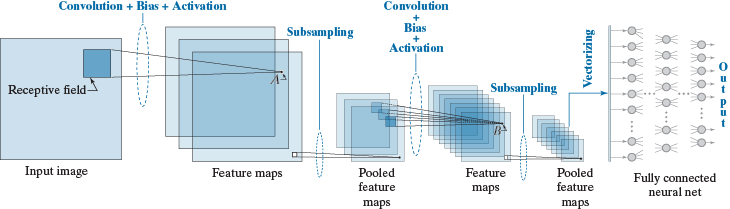
\includegraphics[width=\linewidth]{images/cnn.png}
  \caption{CNN, LeNet architecture}
  \label{fig:cnn}
\end{figure}

\subsubsection{Neural Computations in a CNN\buchSeite{971}}
The convolution value at any point $(x,y)$ is
\[
  w \star a_{x,y} = \sum_l \sum_k w_{l,k} a_{x-l,y-k}
\]
where $l$ and $k$ span the dimension of the kernel $w$.
Assume $w$ is a 3x3, then this expands to
\[
  w \star a_{x,y} = w_{1,1}a_{x-1,y-1} + w_{1,2}a_{x-1,y-2} + \ldots + w_{3,3}a_{x-3,y-3}
\]
Going from 2-D to indexing to 1-D indexing $i=3(l-1)+k$
\[
  w \star a_{x,y} = w_1a_1 + w_2a_2 + \ldots + w_9a_9 = \sum_{i=1}^{9} w_ia_i
\]
To get the usual NN summation for the pre-activation $z$, a bias is added
\[
  z = \sum_{j=1}^{9} w_ja_j + b = w \star a_{x,y} + b
\]
The activation is calculated by running the pre-activation through the activation function
\[
  a = h(z)
\]
\\

Consider a single pixel in a feature map, point $A$ in Fig. \ref{fig:cnn}.
Convolving the receptive field of the input image with the learned 2D filter weights and then adding a learned bias before running the result through an activation function, is identical to the steps performed in a fully connected NN.
What is different though is the fact, that the same learned weights/bias are used for all the pixels in a given feature map.\\

Consider a single pixel in a higher level feature map, point $B$ in Fig. \ref{fig:cnn}.
Since it is the result of convolving three pooled feature maps the calculations contain now the sum of three convolutions
\[
  w_{l,k}^{(1)} \star a_{x,y}^{(1)} + w_{l,k}^{(2)} \star a_{x,y}^{(2)} + w_{l,k}^{(3)} \star a_{x,y}^{(3)} = \sum_l \sum_k w_{l,k}^{(1)}a_{x-l,y-k}^{(1)} + \sum_l \sum_k w_{l,k}^{(2)}a_{x-l,y-k}^{(2)} + \sum_l \sum_k w_{l,k}^{(3)}a_{x-l,y-k}^{(3)}
\]
Nevertheless, each convolution can be written again as a simple sum over a new 1D index.
At the end the sum of these sums is augmented with a bias term and then run through an activation function.

\subsubsection{CNN Forward pass\buchSeite{973}}
Using a layer notation again, the pre-activation at a given pixel is
\[
  z_{x,y}(l) = \sum_l \sum_k w_{l,k}(l) a_{x-l,y-k}(l-1) + b(l) = w(l) \star a_{x,y}(l-1) + b(l)
\]
Hence the activation in a given layer $l$ at a given pixel is
\[
  a_{x,y}(l) = h(z_{x,y}(l))
\]
Note that the book now counts convolutional layers from 1 to $L_c$ which is a slight change in notation (so far, the layer count started at 2).
The convolutional layers start with the input image (possibly multi-dimensional) and stops with the multi-dimensional pooled features
\begin{align*}
  a_{x,y}(0) = \{\text{values of pixels in the input image}(s)\} \\
  a_{x,y}(L_c) = \{\text{values of pooled features in last layer of the CNN}\}
\end{align*}

Pooling layers have no parameters but are needed to reduce the spatial resolution.
For the derivation, we assume that no pooling layers are used, which results in
\begin{table}[h]
	\begin{tabularx}{\textwidth}{llX}
		\textbf{Step} & \textbf{Description} & \textbf{Equations} \\ \hline
		Step 1 & Input images & $\displaystyle a(0) = \text{ the set of image pixels in the input to layer 1}$ \\
		Step 2 & Forward pass & $\displaystyle\text{For each neuron corresponding to location } (x,y) \text{ in each feature map in layer } l \text{ compute:}\newline
    z_{x,y}(l) = w(l) \star a_{x,y}(l-1) + b(l) \text{ and } a_{x,y}(l) = h(z_{x,y}(l)) \text{; } l=1,2,\ldots,L_c$ \\
		\hline
	\end{tabularx}
\end{table}

The fully connected NN at the end of the last convolutional layer is identical to the ones already covered, see Table \ref{tab:forwardPass}.

\subsubsection{CNN Backpropagation\buchSeite{974}}
Since the forward pass is very similar to a fully connected NN, the same is expected for backpropagation:
\begin{align*}
  \frac{\partial E}{\partial b(l)} &= \sum_x \sum_y \delta_{x,y}(l) \\
  w_{l,k}(l) &= w_{l,k}(l) - \alpha \frac{\partial E}{\partial w_{l,k}} = w_{l,k}(l) - \alpha \delta_{l,k}(l) \star \text{rot180}(a(l-1)) \\
  b(l) &= b(l) - \alpha \frac{\partial E}{\partial b(l)} = b(l) - \alpha \sum_x \sum_y \delta_{x,y}(l)
\end{align*}
In the forward pass, the pooling reduced the spatial resolution.
Hence in backpropagation, the resolution needs to be increased.
\begin{itemize}
  \item For average pooling this is achieved by pixel replication, since each high res pixel contributed equally for the low res pixel (e.g., kron(temp,ones(2,2)/4);)
  \item For max pooling this is achieved by remembering which high res pixels won and copy the low res values to those pixels while setting the loser pixels to zero
\end{itemize}
\begin{table}[h]
	\begin{tabularx}{\textwidth}{llX}
		\textbf{Step} & \textbf{Description} & \textbf{Equations} \\ \hline
		Step 1 & Input images & $\displaystyle a(0) = \text{ the set of image pixels in the input to layer 1}$ \\
		Step 2 & Forward pass & $\displaystyle\text{For each neuron corresponding to location } (x,y) \text{ in each feature map in layer } l\newline
    \text{compute: } z_{x,y}(l) = w(l) \star a_{x,y}(l-1) + b(l) \text{ and } a_{x,y}(l) = h(z_{x,y}(l)) \text{; } l=1,2,\ldots,L_c$ \\
    Step 3 & Backpropagation & $\displaystyle\text{For each neuron in each feature map in layer } l \text{ compute:}\newline
    \delta_{x,y}(l) = h'(z_{x,y}(l))[\delta_{x,y}(l+1) \star \text{rot180}(w(l+1))] \text{; } l=L_c-1,L_c-2,\ldots,1$ \\
    Step 4 & Update parameters & $\displaystyle\text{Update the weights and bias for each feature map using }\newline
    w_{l,k}(l) = w_{l,k}(l) - \alpha\delta_{l,k}(l) \star \text{rot180}(\alpha(l-1)) \text{ and } b(l)=b(l) - \alpha\sum_x\sum_y\delta_{x,y}(l) \text{; }\newline
    l=1,2,\ldots,L_c $ \\
		\hline
	\end{tabularx}
\end{table}

%\section{Practical exercises}
\subsection{Morphological Image Processing}
\subsubsection{Exercise 1}
Write a Matlab script that generates a gray-scale image f(x,y) as in problem 9.35 and use the appropriate gray-scale morphological image processing procedure to clean up the spikes.
\textbf{Problem 9.35}
A gray-scale image, $f(x,y)$, is corrupted by nonoverlapping noise spikes, that can be modeled as small, cylindrical artifacts of radii $R_{min}\leq r\leq R_{max}$ and amplitude $A_{min}\leq a \leq A_{max}$.\\
\textbf{Solution}
\begin{lstlisting}
I = imread('rice.png');
subplot(3,3,1);
imshow(I);

for x = 2:9
    S = strel('square',x);
    Iopen = imopen(I,S);
    subplot(3,3,x);
    imshow(Iopen,[]);
end
\end{lstlisting}
\subsubsection{Exercise 2}
Write a Matlab script that generates a bright box on top of a dark background. Now use a simple lowpass filter $(out=filter2(ones(N,N)/N^2,in))$ to smear out the edges of the box. Calculate the gradient magnitude image of this smeard out image and display it for different lowpass filters. Calculate the average gradient magnitude per pixel and graph it relative to the size of the lowpass filter. What do you observe?\\
\textbf{Solution}
\begin{lstlisting}
%Generate dark background
I = zeros(100);
%Generate bright box
I(40:80,30:70) = 1;

subplot(2,5,1);
imshow(I);
title('Original');

M = [5,10,15,20];

for i = 1:4
    N = M(i);
    fsmear = filter2(ones(N,N)/N^2,I);

    subplot(2,5,i+1);
    imshow(fsmear);

    grad = gradient(fsmear);
    subplot(2,5,i+6);
    imshow(grad, []);

    mean(mean(grad))
end
\end{lstlisting}
\textbf{Observation}

\end{document}
